% IEEE Transactions on Radar Systems -- Regular Paper, first submission (IEEEtran journal template).
% R8 (29 Sep 2026): R7 + detection of newly appearing targets, noise-limited whitening gains, persistent-target
% blindness, second radar (JKU 77 GHz), ACI and K-texture baselines. Protocols: repo research/r7c/{detection,jku,baselines}.
% Every numeric result is a macro: generated/r7_macros.tex (repo make_generated.py), generated/submission_macros.tex
% (../analysis_provenance/na_vs_in.py) and generated/r8_macros.tex (../analysis_provenance/make_r8_macros.py).
% Author biographies/photos are required only at the final-files stage: see ../final_stage_only/.
\documentclass[journal]{IEEEtran}
\usepackage[T1]{fontenc}
\usepackage{amsmath,amssymb,amsthm,booktabs,array,graphicx}
\usepackage{cite,xurl,enumitem}
\usepackage[hidelinks]{hyperref}
\graphicspath{{figures/}}
\newtheorem{proposition}{Proposition}
\newtheorem{corollary}{Corollary}
\newcommand{\PP}{\mathbb{P}}
\newcommand{\BelowGOnemEightA}{5}
\newcommand{\BelowGOnemEightB}{0}
\newcommand{\BelowGOnemSixteenA}{4}
\newcommand{\BelowGOnemSixteenB}{0}
\newcommand{\BelowINFourmEightA}{5}
\newcommand{\BelowINFourmEightB}{0}
\newcommand{\BelowINFourmSixteenA}{9}
\newcommand{\BelowINFourmSixteenB}{0}
\newcommand{\BelowINOnemEightA}{0}
\newcommand{\BelowINOnemEightB}{0}
\newcommand{\BelowINOnemSixteenA}{7}
\newcommand{\BelowINOnemSixteenB}{0}
\newcommand{\BelowINTwomEightA}{7}
\newcommand{\BelowINTwomEightB}{0}
\newcommand{\BelowINTwomSixteenA}{4}
\newcommand{\BelowINTwomSixteenB}{0}
\newcommand{\BelowLSmEightA}{2}
\newcommand{\BelowLSmEightB}{0}
\newcommand{\BelowLSmSixteenA}{4}
\newcommand{\BelowLSmSixteenB}{0}
\newcommand{\BelowMLPmEightA}{21}
\newcommand{\BelowMLPmEightB}{0}
\newcommand{\BelowMLPmSixteenA}{21}
\newcommand{\BelowMLPmSixteenB}{0}
\newcommand{\BelowMONmEightA}{4}
\newcommand{\BelowMONmEightB}{0}
\newcommand{\BelowMONmSixteenA}{7}
\newcommand{\BelowMONmSixteenB}{0}
\newcommand{\BelowNAFourGmEightA}{66}
\newcommand{\BelowNAFourGmEightB}{2}
\newcommand{\BelowNAFourGmSixteenA}{29}
\newcommand{\BelowNAFourGmSixteenB}{2}
\newcommand{\BelowNAFourmEightA}{5}
\newcommand{\BelowNAFourmEightB}{0}
\newcommand{\BelowNAFourmSixteenA}{11}
\newcommand{\BelowNAFourmSixteenB}{0}
\newcommand{\BelowNAOneGmEightA}{62}
\newcommand{\BelowNAOneGmEightB}{0}
\newcommand{\BelowNAOneGmSixteenA}{45}
\newcommand{\BelowNAOneGmSixteenB}{2}
\newcommand{\BelowNAOnemEightA}{2}
\newcommand{\BelowNAOnemEightB}{0}
\newcommand{\BelowNAOnemSixteenA}{9}
\newcommand{\BelowNAOnemSixteenB}{0}
\newcommand{\BelowNATwomEightA}{5}
\newcommand{\BelowNATwomEightB}{0}
\newcommand{\BelowNATwomSixteenA}{9}
\newcommand{\BelowNATwomSixteenB}{0}
\newcommand{\BelowRMSmEightA}{29}
\newcommand{\BelowRMSmEightB}{0}
\newcommand{\BelowRMSmSixteenA}{20}
\newcommand{\BelowRMSmSixteenB}{4}
\newcommand{\BelowUmEightA}{25}
\newcommand{\BelowUmEightB}{5}
\newcommand{\BelowUmSixteenA}{21}
\newcommand{\BelowUmSixteenB}{5}
\newcommand{\CFiveCorrA}{0.86}
\newcommand{\CFiveCorrB}{0.96}
\newcommand{\CFiveMaeA}{0.0090}
\newcommand{\CFiveMaeB}{0.0012}
\newcommand{\CFiveNaiveA}{0.0156}
\newcommand{\CFiveNaiveB}{0.0042}
\newcommand{\CleanGOnemEightA}{1.012}
\newcommand{\CleanGOnemEightB}{1.028}
\newcommand{\CleanGOnemSixteenA}{0.997}
\newcommand{\CleanGOnemSixteenB}{0.992}
\newcommand{\CleanINFourmEightA}{0.848}
\newcommand{\CleanINFourmEightB}{0.933}
\newcommand{\CleanINFourmSixteenA}{0.802}
\newcommand{\CleanINFourmSixteenB}{0.820}
\newcommand{\CleanINOnemEightA}{1.000}
\newcommand{\CleanINOnemEightB}{1.000}
\newcommand{\CleanINOnemSixteenA}{1.000}
\newcommand{\CleanINOnemSixteenB}{1.000}
\newcommand{\CleanINTwomEightA}{0.878}
\newcommand{\CleanINTwomEightB}{0.932}
\newcommand{\CleanINTwomSixteenA}{0.865}
\newcommand{\CleanINTwomSixteenB}{0.873}
\newcommand{\CleanLSmEightA}{0.859}
\newcommand{\CleanLSmEightB}{0.967}
\newcommand{\CleanLSmSixteenA}{0.871}
\newcommand{\CleanLSmSixteenB}{1.018}
\newcommand{\CleanMLPmEightA}{1.378}
\newcommand{\CleanMLPmEightB}{1.862}
\newcommand{\CleanMLPmSixteenA}{1.390}
\newcommand{\CleanMLPmSixteenB}{1.740}
\newcommand{\CleanMONmEightA}{0.953}
\newcommand{\CleanMONmEightB}{0.952}
\newcommand{\CleanMONmSixteenA}{0.980}
\newcommand{\CleanMONmSixteenB}{1.002}
\newcommand{\CleanNAFourGmEightA}{0.666}
\newcommand{\CleanNAFourGmEightB}{0.626}
\newcommand{\CleanNAFourGmSixteenA}{0.682}
\newcommand{\CleanNAFourGmSixteenB}{0.654}
\newcommand{\CleanNAFourmEightA}{0.706}
\newcommand{\CleanNAFourmEightB}{0.695}
\newcommand{\CleanNAFourmSixteenA}{0.709}
\newcommand{\CleanNAFourmSixteenB}{0.704}
\newcommand{\CleanNAOneGmEightA}{0.927}
\newcommand{\CleanNAOneGmEightB}{0.873}
\newcommand{\CleanNAOneGmSixteenA}{0.952}
\newcommand{\CleanNAOneGmSixteenB}{0.913}
\newcommand{\CleanNAOnemEightA}{0.985}
\newcommand{\CleanNAOnemEightB}{0.982}
\newcommand{\CleanNAOnemSixteenA}{0.989}
\newcommand{\CleanNAOnemSixteenB}{0.984}
\newcommand{\CleanNATwomEightA}{0.738}
\newcommand{\CleanNATwomEightB}{0.731}
\newcommand{\CleanNATwomSixteenA}{0.739}
\newcommand{\CleanNATwomSixteenB}{0.738}
\newcommand{\CleanRMSmEightA}{1.480}
\newcommand{\CleanRMSmEightB}{1.930}
\newcommand{\CleanRMSmSixteenA}{1.404}
\newcommand{\CleanRMSmSixteenB}{1.729}
\newcommand{\CleanUmEightA}{1.065}
\newcommand{\CleanUmEightB}{1.660}
\newcommand{\CleanUmSixteenA}{1.073}
\newcommand{\CleanUmSixteenB}{1.700}
\newcommand{\CovGOnemEightA}{0.903}
\newcommand{\CovGOnemEightB}{0.991}
\newcommand{\CovGOnemSixteenA}{0.900}
\newcommand{\CovGOnemSixteenB}{0.990}
\newcommand{\CovINFourmEightA}{0.901}
\newcommand{\CovINFourmEightB}{0.991}
\newcommand{\CovINFourmSixteenA}{0.901}
\newcommand{\CovINFourmSixteenB}{0.990}
\newcommand{\CovINOnemEightA}{0.902}
\newcommand{\CovINOnemEightB}{0.991}
\newcommand{\CovINOnemSixteenA}{0.901}
\newcommand{\CovINOnemSixteenB}{0.990}
\newcommand{\CovINTwomEightA}{0.901}
\newcommand{\CovINTwomEightB}{0.991}
\newcommand{\CovINTwomSixteenA}{0.901}
\newcommand{\CovINTwomSixteenB}{0.990}
\newcommand{\CovLSmEightA}{0.899}
\newcommand{\CovLSmEightB}{0.990}
\newcommand{\CovLSmSixteenA}{0.900}
\newcommand{\CovLSmSixteenB}{0.991}
\newcommand{\CovMLPmEightA}{0.898}
\newcommand{\CovMLPmEightB}{0.990}
\newcommand{\CovMLPmSixteenA}{0.901}
\newcommand{\CovMLPmSixteenB}{0.990}
\newcommand{\CovMONmEightA}{0.903}
\newcommand{\CovMONmEightB}{0.993}
\newcommand{\CovMONmSixteenA}{0.904}
\newcommand{\CovMONmSixteenB}{0.992}
\newcommand{\CovMinGOnemEightA}{0.860}
\newcommand{\CovMinGOnemEightB}{0.978}
\newcommand{\CovMinGOnemSixteenA}{0.845}
\newcommand{\CovMinGOnemSixteenB}{0.979}
\newcommand{\CovMinINFourmEightA}{0.873}
\newcommand{\CovMinINFourmEightB}{0.982}
\newcommand{\CovMinINFourmSixteenA}{0.869}
\newcommand{\CovMinINFourmSixteenB}{0.978}
\newcommand{\CovMinINOnemEightA}{0.880}
\newcommand{\CovMinINOnemEightB}{0.980}
\newcommand{\CovMinINOnemSixteenA}{0.864}
\newcommand{\CovMinINOnemSixteenB}{0.973}
\newcommand{\CovMinINTwomEightA}{0.862}
\newcommand{\CovMinINTwomEightB}{0.983}
\newcommand{\CovMinINTwomSixteenA}{0.871}
\newcommand{\CovMinINTwomSixteenB}{0.982}
\newcommand{\CovMinLSmEightA}{0.878}
\newcommand{\CovMinLSmEightB}{0.982}
\newcommand{\CovMinLSmSixteenA}{0.866}
\newcommand{\CovMinLSmSixteenB}{0.981}
\newcommand{\CovMinMLPmEightA}{0.854}
\newcommand{\CovMinMLPmEightB}{0.979}
\newcommand{\CovMinMLPmSixteenA}{0.850}
\newcommand{\CovMinMLPmSixteenB}{0.977}
\newcommand{\CovMinMONmEightA}{0.873}
\newcommand{\CovMinMONmEightB}{0.982}
\newcommand{\CovMinMONmSixteenA}{0.862}
\newcommand{\CovMinMONmSixteenB}{0.984}
\newcommand{\CovMinNAFourGmEightA}{0.806}
\newcommand{\CovMinNAFourGmEightB}{0.968}
\newcommand{\CovMinNAFourGmSixteenA}{0.811}
\newcommand{\CovMinNAFourGmSixteenB}{0.964}
\newcommand{\CovMinNAFourmEightA}{0.873}
\newcommand{\CovMinNAFourmEightB}{0.983}
\newcommand{\CovMinNAFourmSixteenA}{0.853}
\newcommand{\CovMinNAFourmSixteenB}{0.980}
\newcommand{\CovMinNAOneGmEightA}{0.805}
\newcommand{\CovMinNAOneGmEightB}{0.972}
\newcommand{\CovMinNAOneGmSixteenA}{0.812}
\newcommand{\CovMinNAOneGmSixteenB}{0.968}
\newcommand{\CovMinNAOnemEightA}{0.877}
\newcommand{\CovMinNAOnemEightB}{0.980}
\newcommand{\CovMinNAOnemSixteenA}{0.855}
\newcommand{\CovMinNAOnemSixteenB}{0.975}
\newcommand{\CovMinNATwomEightA}{0.866}
\newcommand{\CovMinNATwomEightB}{0.980}
\newcommand{\CovMinNATwomSixteenA}{0.861}
\newcommand{\CovMinNATwomSixteenB}{0.978}
\newcommand{\CovMinRMSmEightA}{0.861}
\newcommand{\CovMinRMSmEightB}{0.979}
\newcommand{\CovMinRMSmSixteenA}{0.845}
\newcommand{\CovMinRMSmSixteenB}{0.963}
\newcommand{\CovMinUmEightA}{0.781}
\newcommand{\CovMinUmEightB}{0.949}
\newcommand{\CovMinUmSixteenA}{0.801}
\newcommand{\CovMinUmSixteenB}{0.967}
\newcommand{\CovNAFourGmEightA}{0.873}
\newcommand{\CovNAFourGmEightB}{0.982}
\newcommand{\CovNAFourGmSixteenA}{0.885}
\newcommand{\CovNAFourGmSixteenB}{0.985}
\newcommand{\CovNAFourmEightA}{0.900}
\newcommand{\CovNAFourmEightB}{0.990}
\newcommand{\CovNAFourmSixteenA}{0.902}
\newcommand{\CovNAFourmSixteenB}{0.991}
\newcommand{\CovNAOneGmEightA}{0.874}
\newcommand{\CovNAOneGmEightB}{0.981}
\newcommand{\CovNAOneGmSixteenA}{0.882}
\newcommand{\CovNAOneGmSixteenB}{0.984}
\newcommand{\CovNAOnemEightA}{0.901}
\newcommand{\CovNAOnemEightB}{0.991}
\newcommand{\CovNAOnemSixteenA}{0.901}
\newcommand{\CovNAOnemSixteenB}{0.990}
\newcommand{\CovNATwomEightA}{0.900}
\newcommand{\CovNATwomEightB}{0.991}
\newcommand{\CovNATwomSixteenA}{0.901}
\newcommand{\CovNATwomSixteenB}{0.991}
\newcommand{\CovRMSmEightA}{0.899}
\newcommand{\CovRMSmEightB}{0.991}
\newcommand{\CovRMSmSixteenA}{0.899}
\newcommand{\CovRMSmSixteenB}{0.989}
\newcommand{\CovUmEightA}{0.899}
\newcommand{\CovUmEightB}{0.989}
\newcommand{\CovUmSixteenA}{0.899}
\newcommand{\CovUmSixteenB}{0.989}
\newcommand{\CurveHighGOnemEightA}{0.918}
\newcommand{\CurveHighGOnemEightB}{0.995}
\newcommand{\CurveHighGOnemSixteenA}{0.908}
\newcommand{\CurveHighGOnemSixteenB}{0.993}
\newcommand{\CurveHighINFourmEightA}{0.902}
\newcommand{\CurveHighINFourmEightB}{0.992}
\newcommand{\CurveHighINFourmSixteenA}{0.903}
\newcommand{\CurveHighINFourmSixteenB}{0.991}
\newcommand{\CurveHighINOnemEightA}{0.917}
\newcommand{\CurveHighINOnemEightB}{0.994}
\newcommand{\CurveHighINOnemSixteenA}{0.908}
\newcommand{\CurveHighINOnemSixteenB}{0.993}
\newcommand{\CurveHighINTwomEightA}{0.902}
\newcommand{\CurveHighINTwomEightB}{0.993}
\newcommand{\CurveHighINTwomSixteenA}{0.902}
\newcommand{\CurveHighINTwomSixteenB}{0.990}
\newcommand{\CurveHighLSmEightA}{0.883}
\newcommand{\CurveHighLSmEightB}{0.986}
\newcommand{\CurveHighLSmSixteenA}{0.890}
\newcommand{\CurveHighLSmSixteenB}{0.987}
\newcommand{\CurveHighMLPmEightA}{0.948}
\newcommand{\CurveHighMLPmEightB}{0.997}
\newcommand{\CurveHighMLPmSixteenA}{0.950}
\newcommand{\CurveHighMLPmSixteenB}{0.995}
\newcommand{\CurveHighMONmEightA}{0.878}
\newcommand{\CurveHighMONmEightB}{0.988}
\newcommand{\CurveHighMONmSixteenA}{0.887}
\newcommand{\CurveHighMONmSixteenB}{0.989}
\newcommand{\CurveHighNAFourGmEightA}{0.863}
\newcommand{\CurveHighNAFourGmEightB}{0.978}
\newcommand{\CurveHighNAFourGmSixteenA}{0.880}
\newcommand{\CurveHighNAFourGmSixteenB}{0.981}
\newcommand{\CurveHighNAFourmEightA}{0.890}
\newcommand{\CurveHighNAFourmEightB}{0.988}
\newcommand{\CurveHighNAFourmSixteenA}{0.898}
\newcommand{\CurveHighNAFourmSixteenB}{0.988}
\newcommand{\CurveHighNAOneGmEightA}{0.887}
\newcommand{\CurveHighNAOneGmEightB}{0.986}
\newcommand{\CurveHighNAOneGmSixteenA}{0.894}
\newcommand{\CurveHighNAOneGmSixteenB}{0.987}
\newcommand{\CurveHighNAOnemEightA}{0.915}
\newcommand{\CurveHighNAOnemEightB}{0.993}
\newcommand{\CurveHighNAOnemSixteenA}{0.911}
\newcommand{\CurveHighNAOnemSixteenB}{0.992}
\newcommand{\CurveHighNATwomEightA}{0.898}
\newcommand{\CurveHighNATwomEightB}{0.991}
\newcommand{\CurveHighNATwomSixteenA}{0.905}
\newcommand{\CurveHighNATwomSixteenB}{0.989}
\newcommand{\CurveHighRMSmEightA}{0.951}
\newcommand{\CurveHighRMSmEightB}{0.997}
\newcommand{\CurveHighRMSmSixteenA}{0.957}
\newcommand{\CurveHighRMSmSixteenB}{0.997}
\newcommand{\CurveHighUmEightA}{0.741}
\newcommand{\CurveHighUmEightB}{0.954}
\newcommand{\CurveHighUmSixteenA}{0.744}
\newcommand{\CurveHighUmSixteenB}{0.953}
\newcommand{\CurveLowGOnemEightA}{0.889}
\newcommand{\CurveLowGOnemEightB}{0.989}
\newcommand{\CurveLowGOnemSixteenA}{0.894}
\newcommand{\CurveLowGOnemSixteenB}{0.988}
\newcommand{\CurveLowINFourmEightA}{0.900}
\newcommand{\CurveLowINFourmEightB}{0.990}
\newcommand{\CurveLowINFourmSixteenA}{0.900}
\newcommand{\CurveLowINFourmSixteenB}{0.989}
\newcommand{\CurveLowINOnemEightA}{0.889}
\newcommand{\CurveLowINOnemEightB}{0.988}
\newcommand{\CurveLowINOnemSixteenA}{0.896}
\newcommand{\CurveLowINOnemSixteenB}{0.988}
\newcommand{\CurveLowINTwomEightA}{0.902}
\newcommand{\CurveLowINTwomEightB}{0.991}
\newcommand{\CurveLowINTwomSixteenA}{0.899}
\newcommand{\CurveLowINTwomSixteenB}{0.989}
\newcommand{\CurveLowLSmEightA}{0.909}
\newcommand{\CurveLowLSmEightB}{0.992}
\newcommand{\CurveLowLSmSixteenA}{0.908}
\newcommand{\CurveLowLSmSixteenB}{0.992}
\newcommand{\CurveLowMLPmEightA}{0.824}
\newcommand{\CurveLowMLPmEightB}{0.980}
\newcommand{\CurveLowMLPmSixteenA}{0.818}
\newcommand{\CurveLowMLPmSixteenB}{0.977}
\newcommand{\CurveLowMONmEightA}{0.927}
\newcommand{\CurveLowMONmEightB}{0.996}
\newcommand{\CurveLowMONmSixteenA}{0.921}
\newcommand{\CurveLowMONmSixteenB}{0.995}
\newcommand{\CurveLowNAFourGmEightA}{0.893}
\newcommand{\CurveLowNAFourGmEightB}{0.986}
\newcommand{\CurveLowNAFourGmSixteenA}{0.899}
\newcommand{\CurveLowNAFourGmSixteenB}{0.987}
\newcommand{\CurveLowNAFourmEightA}{0.918}
\newcommand{\CurveLowNAFourmEightB}{0.993}
\newcommand{\CurveLowNAFourmSixteenA}{0.916}
\newcommand{\CurveLowNAFourmSixteenB}{0.993}
\newcommand{\CurveLowNAOneGmEightA}{0.865}
\newcommand{\CurveLowNAOneGmEightB}{0.978}
\newcommand{\CurveLowNAOneGmSixteenA}{0.877}
\newcommand{\CurveLowNAOneGmSixteenB}{0.981}
\newcommand{\CurveLowNAOnemEightA}{0.895}
\newcommand{\CurveLowNAOnemEightB}{0.989}
\newcommand{\CurveLowNAOnemSixteenA}{0.898}
\newcommand{\CurveLowNAOnemSixteenB}{0.988}
\newcommand{\CurveLowNATwomEightA}{0.910}
\newcommand{\CurveLowNATwomEightB}{0.991}
\newcommand{\CurveLowNATwomSixteenA}{0.907}
\newcommand{\CurveLowNATwomSixteenB}{0.991}
\newcommand{\CurveLowRMSmEightA}{0.820}
\newcommand{\CurveLowRMSmEightB}{0.981}
\newcommand{\CurveLowRMSmSixteenA}{0.812}
\newcommand{\CurveLowRMSmSixteenB}{0.974}
\newcommand{\CurveLowUmEightA}{0.982}
\newcommand{\CurveLowUmEightB}{0.999}
\newcommand{\CurveLowUmSixteenA}{0.978}
\newcommand{\CurveLowUmSixteenB}{0.999}
\newcommand{\HoCovGOne}{0.945}
\newcommand{\HoCovINFour}{0.906}
\newcommand{\HoCovINOne}{0.910}
\newcommand{\HoCovINTwo}{0.906}
\newcommand{\HoCovLS}{0.919}
\newcommand{\HoCovMLP}{0.903}
\newcommand{\HoCovMON}{0.896}
\newcommand{\HoCovNAFour}{0.893}
\newcommand{\HoCovNAFourG}{0.856}
\newcommand{\HoCovNAOne}{0.903}
\newcommand{\HoCovNATwo}{0.895}
\newcommand{\HoCovRMS}{0.887}
\newcommand{\HoCovU}{0.859}
\newcommand{\HoMonInf}{infinite}
\newcommand{\HoRatioGOne}{1.104}
\newcommand{\HoRatioINFour}{0.515}
\newcommand{\HoRatioINOne}{1.000}
\newcommand{\HoRatioINTwo}{0.572}
\newcommand{\HoRatioLS}{0.662}
\newcommand{\HoRatioMLP}{2.158}
\newcommand{\HoRatioMON}{0.981}
\newcommand{\HoRatioNAFour}{0.498}
\newcommand{\HoRatioNAFourG}{0.472}
\newcommand{\HoRatioNAOne}{0.921}
\newcommand{\HoRatioNATwo}{0.533}
\newcommand{\HoRatioRMS}{1.243}
\newcommand{\HoRatioU}{1.161}
\newcommand{\MaxdevGOnemEightA}{0.038}
\newcommand{\MaxdevGOnemEightB}{0.011}
\newcommand{\MaxdevGOnemSixteenA}{0.034}
\newcommand{\MaxdevGOnemSixteenB}{0.011}
\newcommand{\MaxdevINFourmEightA}{0.031}
\newcommand{\MaxdevINFourmEightB}{0.010}
\newcommand{\MaxdevINFourmSixteenA}{0.032}
\newcommand{\MaxdevINFourmSixteenB}{0.011}
\newcommand{\MaxdevINOneWFiveTwelve}{0.035}
\newcommand{\MaxdevINOneWTwentyFortyEight}{0.033}
\newcommand{\MaxdevINOnemEightA}{0.037}
\newcommand{\MaxdevINOnemEightB}{0.011}
\newcommand{\MaxdevINOnemSixteenA}{0.036}
\newcommand{\MaxdevINOnemSixteenB}{0.011}
\newcommand{\MaxdevINTwomEightA}{0.035}
\newcommand{\MaxdevINTwomEightB}{0.010}
\newcommand{\MaxdevINTwomSixteenA}{0.034}
\newcommand{\MaxdevINTwomSixteenB}{0.010}
\newcommand{\MaxdevLSmEightA}{0.039}
\newcommand{\MaxdevLSmEightB}{0.012}
\newcommand{\MaxdevLSmSixteenA}{0.039}
\newcommand{\MaxdevLSmSixteenB}{0.012}
\newcommand{\MaxdevMLPWFiveTwelve}{0.103}
\newcommand{\MaxdevMLPWTwentyFortyEight}{0.080}
\newcommand{\MaxdevMLPmEightA}{0.092}
\newcommand{\MaxdevMLPmEightB}{0.015}
\newcommand{\MaxdevMLPmSixteenA}{0.096}
\newcommand{\MaxdevMLPmSixteenB}{0.019}
\newcommand{\MaxdevMONWFiveTwelve}{0.042}
\newcommand{\MaxdevMONWTwentyFortyEight}{0.039}
\newcommand{\MaxdevMONmEightA}{0.043}
\newcommand{\MaxdevMONmEightB}{0.010}
\newcommand{\MaxdevMONmSixteenA}{0.043}
\newcommand{\MaxdevMONmSixteenB}{0.011}
\newcommand{\MaxdevNAFourGmEightA}{0.063}
\newcommand{\MaxdevNAFourGmEightB}{0.020}
\newcommand{\MaxdevNAFourGmSixteenA}{0.049}
\newcommand{\MaxdevNAFourGmSixteenB}{0.016}
\newcommand{\MaxdevNAFourWFiveTwelve}{0.043}
\newcommand{\MaxdevNAFourWTwentyFortyEight}{0.043}
\newcommand{\MaxdevNAFourmEightA}{0.043}
\newcommand{\MaxdevNAFourmEightB}{0.010}
\newcommand{\MaxdevNAFourmSixteenA}{0.043}
\newcommand{\MaxdevNAFourmSixteenB}{0.011}
\newcommand{\MaxdevNAOneGmEightA}{0.062}
\newcommand{\MaxdevNAOneGmEightB}{0.021}
\newcommand{\MaxdevNAOneGmSixteenA}{0.051}
\newcommand{\MaxdevNAOneGmSixteenB}{0.017}
\newcommand{\MaxdevNAOnemEightA}{0.043}
\newcommand{\MaxdevNAOnemEightB}{0.012}
\newcommand{\MaxdevNAOnemSixteenA}{0.042}
\newcommand{\MaxdevNAOnemSixteenB}{0.011}
\newcommand{\MaxdevNATwomEightA}{0.042}
\newcommand{\MaxdevNATwomEightB}{0.011}
\newcommand{\MaxdevNATwomSixteenA}{0.044}
\newcommand{\MaxdevNATwomSixteenB}{0.011}
\newcommand{\MaxdevRMSWFiveTwelve}{0.110}
\newcommand{\MaxdevRMSWTwentyFortyEight}{0.086}
\newcommand{\MaxdevRMSmEightA}{0.096}
\newcommand{\MaxdevRMSmEightB}{0.015}
\newcommand{\MaxdevRMSmSixteenA}{0.103}
\newcommand{\MaxdevRMSmSixteenB}{0.021}
\newcommand{\MaxdevUWFiveTwelve}{0.181}
\newcommand{\MaxdevUWTwentyFortyEight}{0.141}
\newcommand{\MaxdevUmEightA}{0.170}
\newcommand{\MaxdevUmEightB}{0.038}
\newcommand{\MaxdevUmSixteenA}{0.165}
\newcommand{\MaxdevUmSixteenB}{0.039}
\newcommand{\NCleanConf}{39}
\newcommand{\NNoisyConf}{17}
\newcommand{\NUnitsConf}{56}
\newcommand{\NoisyGOnemEightA}{0.979}
\newcommand{\NoisyGOnemEightB}{0.949}
\newcommand{\NoisyGOnemSixteenA}{0.990}
\newcommand{\NoisyGOnemSixteenB}{0.993}
\newcommand{\NoisyINFourmEightA}{0.986}
\newcommand{\NoisyINFourmEightB}{1.228}
\newcommand{\NoisyINFourmSixteenA}{0.953}
\newcommand{\NoisyINFourmSixteenB}{0.964}
\newcommand{\NoisyINOnemEightA}{1.000}
\newcommand{\NoisyINOnemEightB}{1.000}
\newcommand{\NoisyINOnemSixteenA}{1.000}
\newcommand{\NoisyINOnemSixteenB}{1.000}
\newcommand{\NoisyINTwomEightA}{0.977}
\newcommand{\NoisyINTwomEightB}{1.008}
\newcommand{\NoisyINTwomSixteenA}{0.968}
\newcommand{\NoisyINTwomSixteenB}{0.957}
\newcommand{\NoisyLSmEightA}{0.997}
\newcommand{\NoisyLSmEightB}{1.093}
\newcommand{\NoisyLSmSixteenA}{1.046}
\newcommand{\NoisyLSmSixteenB}{1.207}
\newcommand{\NoisyMLPmEightA}{1.178}
\newcommand{\NoisyMLPmEightB}{1.227}
\newcommand{\NoisyMLPmSixteenA}{1.224}
\newcommand{\NoisyMLPmSixteenB}{1.278}
\newcommand{\NoisyMONmEightA}{0.953}
\newcommand{\NoisyMONmEightB}{0.905}
\newcommand{\NoisyMONmSixteenA}{0.980}
\newcommand{\NoisyMONmSixteenB}{0.987}
\newcommand{\NoisyNAFourGmEightA}{0.804}
\newcommand{\NoisyNAFourGmEightB}{0.722}
\newcommand{\NoisyNAFourGmSixteenA}{0.839}
\newcommand{\NoisyNAFourGmSixteenB}{0.811}
\newcommand{\NoisyNAFourmEightA}{0.839}
\newcommand{\NoisyNAFourmEightB}{0.758}
\newcommand{\NoisyNAFourmSixteenA}{0.866}
\newcommand{\NoisyNAFourmSixteenB}{0.840}
\newcommand{\NoisyNAOneGmEightA}{0.851}
\newcommand{\NoisyNAOneGmEightB}{0.764}
\newcommand{\NoisyNAOneGmSixteenA}{0.882}
\newcommand{\NoisyNAOneGmSixteenB}{0.853}
\newcommand{\NoisyNAOnemEightA}{0.897}
\newcommand{\NoisyNAOnemEightB}{0.823}
\newcommand{\NoisyNAOnemSixteenA}{0.915}
\newcommand{\NoisyNAOnemSixteenB}{0.884}
\newcommand{\NoisyNATwomEightA}{0.845}
\newcommand{\NoisyNATwomEightB}{0.763}
\newcommand{\NoisyNATwomSixteenA}{0.871}
\newcommand{\NoisyNATwomSixteenB}{0.843}
\newcommand{\NoisyRMSmEightA}{1.274}
\newcommand{\NoisyRMSmEightB}{1.302}
\newcommand{\NoisyRMSmSixteenA}{1.288}
\newcommand{\NoisyRMSmSixteenB}{1.363}
\newcommand{\NoisyUmEightA}{0.962}
\newcommand{\NoisyUmEightB}{0.951}
\newcommand{\NoisyUmSixteenA}{0.994}
\newcommand{\NoisyUmSixteenB}{1.066}
\newcommand{\RatioGOnemEightA}{1.001}
\newcommand{\RatioGOnemEightB}{1.002}
\newcommand{\RatioGOnemSixteenA}{0.995}
\newcommand{\RatioGOnemSixteenB}{0.993}
\newcommand{\RatioHiGOnemEightA}{1.013}
\newcommand{\RatioHiGOnemEightB}{1.031}
\newcommand{\RatioHiGOnemSixteenA}{1.002}
\newcommand{\RatioHiGOnemSixteenB}{1.005}
\newcommand{\RatioHiINFourmEightA}{0.957}
\newcommand{\RatioHiINFourmEightB}{1.142}
\newcommand{\RatioHiINFourmSixteenA}{0.905}
\newcommand{\RatioHiINFourmSixteenB}{0.918}
\newcommand{\RatioHiINOnemEightA}{1.000}
\newcommand{\RatioHiINOnemEightB}{1.000}
\newcommand{\RatioHiINOnemSixteenA}{1.000}
\newcommand{\RatioHiINOnemSixteenB}{1.000}
\newcommand{\RatioHiINTwomEightA}{0.965}
\newcommand{\RatioHiINTwomEightB}{1.007}
\newcommand{\RatioHiINTwomSixteenA}{0.953}
\newcommand{\RatioHiINTwomSixteenB}{0.953}
\newcommand{\RatioHiLSmEightA}{0.958}
\newcommand{\RatioHiLSmEightB}{1.064}
\newcommand{\RatioHiLSmSixteenA}{0.990}
\newcommand{\RatioHiLSmSixteenB}{1.147}
\newcommand{\RatioHiMLPmEightA}{1.416}
\newcommand{\RatioHiMLPmEightB}{1.839}
\newcommand{\RatioHiMLPmSixteenA}{1.439}
\newcommand{\RatioHiMLPmSixteenB}{1.780}
\newcommand{\RatioHiMONmEightA}{0.963}
\newcommand{\RatioHiMONmEightB}{0.958}
\newcommand{\RatioHiMONmSixteenA}{0.984}
\newcommand{\RatioHiMONmSixteenB}{1.006}
\newcommand{\RatioHiNAFourGmEightA}{0.764}
\newcommand{\RatioHiNAFourGmEightB}{0.697}
\newcommand{\RatioHiNAFourGmSixteenA}{0.787}
\newcommand{\RatioHiNAFourGmSixteenB}{0.758}
\newcommand{\RatioHiNAFourmEightA}{0.800}
\newcommand{\RatioHiNAFourmEightB}{0.738}
\newcommand{\RatioHiNAFourmSixteenA}{0.815}
\newcommand{\RatioHiNAFourmSixteenB}{0.798}
\newcommand{\RatioHiNAOneGmEightA}{0.931}
\newcommand{\RatioHiNAOneGmEightB}{0.876}
\newcommand{\RatioHiNAOneGmSixteenA}{0.958}
\newcommand{\RatioHiNAOneGmSixteenB}{0.920}
\newcommand{\RatioHiNAOnemEightA}{0.988}
\newcommand{\RatioHiNAOnemEightB}{0.989}
\newcommand{\RatioHiNAOnemSixteenA}{0.994}
\newcommand{\RatioHiNAOnemSixteenB}{0.989}
\newcommand{\RatioHiNATwomEightA}{0.808}
\newcommand{\RatioHiNATwomEightB}{0.752}
\newcommand{\RatioHiNATwomSixteenA}{0.824}
\newcommand{\RatioHiNATwomSixteenB}{0.806}
\newcommand{\RatioHiRMSmEightA}{1.507}
\newcommand{\RatioHiRMSmEightB}{1.871}
\newcommand{\RatioHiRMSmSixteenA}{1.449}
\newcommand{\RatioHiRMSmSixteenB}{1.782}
\newcommand{\RatioHiUmEightA}{1.071}
\newcommand{\RatioHiUmEightB}{1.627}
\newcommand{\RatioHiUmSixteenA}{1.085}
\newcommand{\RatioHiUmSixteenB}{1.720}
\newcommand{\RatioINFourmEightA}{0.890}
\newcommand{\RatioINFourmEightB}{1.019}
\newcommand{\RatioINFourmSixteenA}{0.845}
\newcommand{\RatioINFourmSixteenB}{0.861}
\newcommand{\RatioINOnemEightA}{1.000}
\newcommand{\RatioINOnemEightB}{1.000}
\newcommand{\RatioINOnemSixteenA}{1.000}
\newcommand{\RatioINOnemSixteenB}{1.000}
\newcommand{\RatioINTwomEightA}{0.909}
\newcommand{\RatioINTwomEightB}{0.956}
\newcommand{\RatioINTwomSixteenA}{0.895}
\newcommand{\RatioINTwomSixteenB}{0.898}
\newcommand{\RatioLSmEightA}{0.901}
\newcommand{\RatioLSmEightB}{1.005}
\newcommand{\RatioLSmSixteenA}{0.921}
\newcommand{\RatioLSmSixteenB}{1.072}
\newcommand{\RatioLoGOnemEightA}{0.987}
\newcommand{\RatioLoGOnemEightB}{0.968}
\newcommand{\RatioLoGOnemSixteenA}{0.988}
\newcommand{\RatioLoGOnemSixteenB}{0.979}
\newcommand{\RatioLoINFourmEightA}{0.844}
\newcommand{\RatioLoINFourmEightB}{0.935}
\newcommand{\RatioLoINFourmSixteenA}{0.805}
\newcommand{\RatioLoINFourmSixteenB}{0.822}
\newcommand{\RatioLoINOnemEightA}{1.000}
\newcommand{\RatioLoINOnemEightB}{1.000}
\newcommand{\RatioLoINOnemSixteenA}{1.000}
\newcommand{\RatioLoINOnemSixteenB}{1.000}
\newcommand{\RatioLoINTwomEightA}{0.867}
\newcommand{\RatioLoINTwomEightB}{0.918}
\newcommand{\RatioLoINTwomSixteenA}{0.855}
\newcommand{\RatioLoINTwomSixteenB}{0.857}
\newcommand{\RatioLoLSmEightA}{0.863}
\newcommand{\RatioLoLSmEightB}{0.968}
\newcommand{\RatioLoLSmSixteenA}{0.875}
\newcommand{\RatioLoLSmSixteenB}{1.019}
\newcommand{\RatioLoMLPmEightA}{1.257}
\newcommand{\RatioLoMLPmEightB}{1.475}
\newcommand{\RatioLoMLPmSixteenA}{1.288}
\newcommand{\RatioLoMLPmSixteenB}{1.489}
\newcommand{\RatioLoMONmEightA}{0.941}
\newcommand{\RatioLoMONmEightB}{0.909}
\newcommand{\RatioLoMONmSixteenA}{0.975}
\newcommand{\RatioLoMONmSixteenB}{0.988}
\newcommand{\RatioLoNAFourGmEightA}{0.672}
\newcommand{\RatioLoNAFourGmEightB}{0.629}
\newcommand{\RatioLoNAFourGmSixteenA}{0.687}
\newcommand{\RatioLoNAFourGmSixteenB}{0.659}
\newcommand{\RatioLoNAFourmEightA}{0.713}
\newcommand{\RatioLoNAFourmEightB}{0.701}
\newcommand{\RatioLoNAFourmSixteenA}{0.714}
\newcommand{\RatioLoNAFourmSixteenB}{0.706}
\newcommand{\RatioLoNAOneGmEightA}{0.866}
\newcommand{\RatioLoNAOneGmEightB}{0.787}
\newcommand{\RatioLoNAOneGmSixteenA}{0.895}
\newcommand{\RatioLoNAOneGmSixteenB}{0.860}
\newcommand{\RatioLoNAOnemEightA}{0.913}
\newcommand{\RatioLoNAOnemEightB}{0.853}
\newcommand{\RatioLoNAOnemSixteenA}{0.930}
\newcommand{\RatioLoNAOnemSixteenB}{0.907}
\newcommand{\RatioLoNATwomEightA}{0.747}
\newcommand{\RatioLoNATwomEightB}{0.724}
\newcommand{\RatioLoNATwomSixteenA}{0.748}
\newcommand{\RatioLoNATwomSixteenB}{0.745}
\newcommand{\RatioLoRMSmEightA}{1.364}
\newcommand{\RatioLoRMSmEightB}{1.565}
\newcommand{\RatioLoRMSmSixteenA}{1.320}
\newcommand{\RatioLoRMSmSixteenB}{1.533}
\newcommand{\RatioLoUmEightA}{0.985}
\newcommand{\RatioLoUmEightB}{1.140}
\newcommand{\RatioLoUmSixteenA}{1.010}
\newcommand{\RatioLoUmSixteenB}{1.261}
\newcommand{\RatioMLPmEightA}{1.310}
\newcommand{\RatioMLPmEightB}{1.628}
\newcommand{\RatioMLPmSixteenA}{1.337}
\newcommand{\RatioMLPmSixteenB}{1.585}
\newcommand{\RatioMONmEightA}{0.953}
\newcommand{\RatioMONmEightB}{0.936}
\newcommand{\RatioMONmSixteenA}{0.980}
\newcommand{\RatioMONmSixteenB}{0.998}
\newcommand{\RatioNAFourGmEightA}{0.707}
\newcommand{\RatioNAFourGmEightB}{0.656}
\newcommand{\RatioNAFourGmSixteenA}{0.726}
\newcommand{\RatioNAFourGmSixteenB}{0.698}
\newcommand{\RatioNAFourmEightA}{0.746}
\newcommand{\RatioNAFourmEightB}{0.715}
\newcommand{\RatioNAFourmSixteenA}{0.753}
\newcommand{\RatioNAFourmSixteenB}{0.743}
\newcommand{\RatioNAOneGmEightA}{0.902}
\newcommand{\RatioNAOneGmEightB}{0.836}
\newcommand{\RatioNAOneGmSixteenA}{0.930}
\newcommand{\RatioNAOneGmSixteenB}{0.894}
\newcommand{\RatioNAOnemEightA}{0.955}
\newcommand{\RatioNAOnemEightB}{0.928}
\newcommand{\RatioNAOnemSixteenA}{0.966}
\newcommand{\RatioNAOnemSixteenB}{0.952}
\newcommand{\RatioNATwomEightA}{0.771}
\newcommand{\RatioNATwomEightB}{0.741}
\newcommand{\RatioNATwomSixteenA}{0.777}
\newcommand{\RatioNATwomSixteenB}{0.769}
\newcommand{\RatioRMSmEightA}{1.410}
\newcommand{\RatioRMSmEightB}{1.701}
\newcommand{\RatioRMSmSixteenA}{1.368}
\newcommand{\RatioRMSmSixteenB}{1.609}
\newcommand{\RatioUmEightA}{1.031}
\newcommand{\RatioUmEightB}{1.388}
\newcommand{\RatioUmSixteenA}{1.048}
\newcommand{\RatioUmSixteenB}{1.475}
\newcommand{\RefGOnemEightA}{0.029}
\newcommand{\RefGOnemEightB}{0.009}
\newcommand{\RefGOnemSixteenA}{0.029}
\newcommand{\RefGOnemSixteenB}{0.009}
\newcommand{\RefINFourmEightA}{0.029}
\newcommand{\RefINFourmEightB}{0.009}
\newcommand{\RefINFourmSixteenA}{0.029}
\newcommand{\RefINFourmSixteenB}{0.009}
\newcommand{\RefINOnemEightA}{0.029}
\newcommand{\RefINOnemEightB}{0.009}
\newcommand{\RefINOnemSixteenA}{0.029}
\newcommand{\RefINOnemSixteenB}{0.009}
\newcommand{\RefINTwomEightA}{0.029}
\newcommand{\RefINTwomEightB}{0.009}
\newcommand{\RefINTwomSixteenA}{0.029}
\newcommand{\RefINTwomSixteenB}{0.009}
\newcommand{\RefLSmEightA}{0.029}
\newcommand{\RefLSmEightB}{0.009}
\newcommand{\RefLSmSixteenA}{0.029}
\newcommand{\RefLSmSixteenB}{0.009}
\newcommand{\RefMLPmEightA}{0.029}
\newcommand{\RefMLPmEightB}{0.009}
\newcommand{\RefMLPmSixteenA}{0.029}
\newcommand{\RefMLPmSixteenB}{0.009}
\newcommand{\RefMONmEightA}{0.029}
\newcommand{\RefMONmEightB}{0.009}
\newcommand{\RefMONmSixteenA}{0.029}
\newcommand{\RefMONmSixteenB}{0.009}
\newcommand{\RefNAFourGmEightA}{0.029}
\newcommand{\RefNAFourGmEightB}{0.009}
\newcommand{\RefNAFourGmSixteenA}{0.029}
\newcommand{\RefNAFourGmSixteenB}{0.009}
\newcommand{\RefNAFourmEightA}{0.029}
\newcommand{\RefNAFourmEightB}{0.009}
\newcommand{\RefNAFourmSixteenA}{0.029}
\newcommand{\RefNAFourmSixteenB}{0.009}
\newcommand{\RefNAOneGmEightA}{0.029}
\newcommand{\RefNAOneGmEightB}{0.009}
\newcommand{\RefNAOneGmSixteenA}{0.029}
\newcommand{\RefNAOneGmSixteenB}{0.009}
\newcommand{\RefNAOnemEightA}{0.029}
\newcommand{\RefNAOnemEightB}{0.009}
\newcommand{\RefNAOnemSixteenA}{0.029}
\newcommand{\RefNAOnemSixteenB}{0.009}
\newcommand{\RefNATwomEightA}{0.029}
\newcommand{\RefNATwomEightB}{0.009}
\newcommand{\RefNATwomSixteenA}{0.029}
\newcommand{\RefNATwomSixteenB}{0.009}
\newcommand{\RefRMSmEightA}{0.029}
\newcommand{\RefRMSmEightB}{0.009}
\newcommand{\RefRMSmSixteenA}{0.029}
\newcommand{\RefRMSmSixteenB}{0.009}
\newcommand{\RefUmEightA}{0.029}
\newcommand{\RefUmEightB}{0.009}
\newcommand{\RefUmSixteenA}{0.029}
\newcommand{\RefUmSixteenB}{0.009}
\newcommand{\SynNaGCov}{0.884}
\newcommand{\SynNaHigh}{0.899}
\newcommand{\SynNaLow}{0.904}
\newcommand{\SynNaRatio}{0.949}
\newcommand{\SynNoiseInHigh}{0.909}
\newcommand{\SynNoiseInLow}{0.890}
\newcommand{\SynNoiseMaxT}{1.72}
\newcommand{\SynNoiseMonHigh}{0.882}
\newcommand{\SynNoiseMonLow}{0.926}
\newcommand{\SynNuHat}{1.000}
\newcommand{\SynReps}{200}
\newcommand{\SynRhoHat}{0.930}
\newcommand{\SynSirvInHigh}{0.901}
\newcommand{\SynSirvInLow}{0.900}
\newcommand{\SynSirvMaxT}{1.39}
\newcommand{\SynSirvMonHigh}{0.885}
\newcommand{\SynSirvMonLow}{0.912}
\newcommand{\TrRatioINFour}{0.993}
\newcommand{\TrRatioINOne}{1.000}
\newcommand{\TrRatioLS}{0.967}
\newcommand{\TrRatioMLP}{1.200}
\newcommand{\TrRatioNAFour}{0.936}
\newcommand{\TrRatioNAFourG}{0.893}
\newcommand{\TrRatioRMS}{1.466}
\newcommand{\TrRatioU}{1.470}
\newcommand{\TrWorstINFour}{0.894}
\newcommand{\TrWorstINOne}{0.882}
\newcommand{\TrWorstLS}{0.774}
\newcommand{\TrWorstMLP}{0.622}
\newcommand{\TrWorstNAFour}{0.863}
\newcommand{\TrWorstNAFourG}{0.842}
\newcommand{\TrWorstRMS}{0.681}
\newcommand{\TrWorstU}{0.716}

% Added for the T-RS submission (29 Sep 2026). Source: ../analysis_provenance/na_vs_in.py and
% na_vs_in_output.txt (confirmatory rotations 2-3, 56 units, day-cluster bootstrap, 10,000 resamples).
% Clean/noisy same-order ratios are exact quotients of the subgroup geometric means in r7_macros.tex.
\newcommand{\SameNAFourA}{0.891}\newcommand{\SameLoNAFourA}{0.872}\newcommand{\SameHiNAFourA}{0.905}
\newcommand{\SameNAFourB}{0.863}\newcommand{\SameLoNAFourB}{0.852}\newcommand{\SameHiNAFourB}{0.871}
\newcommand{\SameNATwoA}{0.868}\newcommand{\SameLoNATwoA}{0.830}\newcommand{\SameHiNATwoA}{0.885}
\newcommand{\SameNAFourEightA}{0.839}\newcommand{\SameLoNAFourEightA}{0.815}\newcommand{\SameHiNAFourEightA}{0.853}
\newcommand{\SameNAFourClean}{0.884}\newcommand{\SameNAFourNoisy}{0.909}

% Generated by analysis_provenance/make_r8_macros.py from the saved R8 results. Do not edit.
\newcommand{\ACIDev}{0.015}
\newcommand{\ACIDevSplit}{0.024}
\newcommand{\ACIRadius}{1.000}
\newcommand{\ACIWithin}{0.9007}
\newcommand{\ACIWithinSplit}{0.9013}
\newcommand{\ACIWorst}{0.897}
\newcommand{\ACIWorstSplit}{0.882}
\newcommand{\BOneRatio}{1.009}
\newcommand{\BOneRatioHi}{1.011}
\newcommand{\BOneRatioLo}{1.006}
\newcommand{\DetINFourGainCAHalf}{7.4}
\newcommand{\DetINFourGainCAHiHalf}{9.5}
\newcommand{\DetINFourGainCAHiNinety}{11.0}
\newcommand{\DetINFourGainCALoHalf}{4.5}
\newcommand{\DetINFourGainCALoNinety}{4.9}
\newcommand{\DetINFourGainCANinety}{8.3}
\newcommand{\DetINFourGainLocHalf}{10.2}
\newcommand{\DetINFourGainLocHiHalf}{13.3}
\newcommand{\DetINFourGainLocHiNinety}{12.6}
\newcommand{\DetINFourGainLocLoHalf}{6.7}
\newcommand{\DetINFourGainLocLoNinety}{5.9}
\newcommand{\DetINFourGainLocNinety}{9.7}
\newcommand{\DetINFourScrHalf}{-1.3}
\newcommand{\DetINFourScrNinety}{8.0}
\newcommand{\DetINGainCAHalf}{7.0}
\newcommand{\DetINGainCAHiHalf}{9.0}
\newcommand{\DetINGainCAHiNinety}{10.0}
\newcommand{\DetINGainCALoHalf}{4.3}
\newcommand{\DetINGainCALoNinety}{4.6}
\newcommand{\DetINGainCANinety}{7.6}
\newcommand{\DetINGainLocHalf}{9.8}
\newcommand{\DetINGainLocHiHalf}{12.6}
\newcommand{\DetINGainLocHiNinety}{11.7}
\newcommand{\DetINGainLocLoHalf}{6.4}
\newcommand{\DetINGainLocLoNinety}{5.6}
\newcommand{\DetINGainLocNinety}{9.0}
\newcommand{\DetINScrHalf}{-0.9}
\newcommand{\DetINScrNinety}{8.7}
\newcommand{\DetMae}{0.021}
\newcommand{\DetMaePooled}{0.010}
\newcommand{\DetNAFourGainCAHalf}{8.0}
\newcommand{\DetNAFourGainCAHiHalf}{10.0}
\newcommand{\DetNAFourGainCAHiNinety}{12.5}
\newcommand{\DetNAFourGainCALoHalf}{5.5}
\newcommand{\DetNAFourGainCALoNinety}{6.3}
\newcommand{\DetNAFourGainCANinety}{9.8}
\newcommand{\DetNAFourGainLocHalf}{10.9}
\newcommand{\DetNAFourGainLocHiHalf}{13.7}
\newcommand{\DetNAFourGainLocHiNinety}{14.1}
\newcommand{\DetNAFourGainLocLoHalf}{7.6}
\newcommand{\DetNAFourGainLocLoNinety}{7.3}
\newcommand{\DetNAFourGainLocNinety}{11.2}
\newcommand{\DetNAFourScrHalf}{-1.9}
\newcommand{\DetNAFourScrNinety}{6.5}
\newcommand{\DetNTest}{74{,}980}
\newcommand{\DetNaiveGain}{11.2}
\newcommand{\DetPfaCASixteen}{0.0103}
\newcommand{\DetPfaCAloc}{0.0110}
\newcommand{\DetPfaINOne}{0.0099}
\newcommand{\DetPfaNAFour}{0.0095}
\newcommand{\DetPfaNAFourG}{0.0151}
\newcommand{\DetPfaNAFourGmilli}{0.0028}
\newcommand{\DetScrErrAbs}{0.9}
\newcommand{\DwCAlocEight}{8.0}
\newcommand{\DwCAlocOne}{9.0}
\newcommand{\DwIN}{10.7}
\newcommand{\DwINHi}{13.4}
\newcommand{\DwINLo}{7.4}
\newcommand{\DwINNinety}{9.4}
\newcommand{\DwNAFour}{11.7}
\newcommand{\DwNAFourHi}{13.8}
\newcommand{\DwNAFourLo}{9.2}
\newcommand{\DwNAFourNinety}{14.0}
\newcommand{\JDevIN}{0.066}
\newcommand{\JDevNAFour}{0.055}
\newcommand{\JDevNAOne}{0.067}
\newcommand{\JFourHit}{0.792}
\newcommand{\JFourIN}{0.901}
\newcommand{\JFourNAFour}{0.870}
\newcommand{\JFourNAOne}{0.828}
\newcommand{\JFourRate}{2.0}
\newcommand{\JGenHigh}{7.5}
\newcommand{\JGenLow}{-0.7}
\newcommand{\JGenMid}{4.5}
\newcommand{\JINGainHigh}{3.11}
\newcommand{\JINGainLow}{-1.45}
\newcommand{\JINGainMid}{0.02}
\newcommand{\JInHigh}{0.962}
\newcommand{\JInLow}{0.897}
\newcommand{\JMae}{0.010}
\newcommand{\JMaeB}{0.002}
\newcommand{\JMeasTop}{5.8}
\newcommand{\JNAFourGainHigh}{7.03}
\newcommand{\JNAFourGainLow}{-1.26}
\newcommand{\JNAFourGainMid}{1.33}
\newcommand{\JNTest}{1.32}
\newcommand{\JPredHigh}{0.932}
\newcommand{\JUHigh}{0.017}
\newcommand{\JULow}{0.972}
\newcommand{\OnCAloc}{0.56}
\newcommand{\OnCumPfaCAloc}{0.031}
\newcommand{\OnCumPfaIN}{0.068}
\newcommand{\OnGainIN}{8.4}
\newcommand{\OnGainINHi}{11.1}
\newcommand{\OnGainINLo}{5.2}
\newcommand{\OnGainNAFour}{9.4}
\newcommand{\OnGainNAFourHi}{11.3}
\newcommand{\OnGainNAFourLo}{7.2}
\newcommand{\OnGainOneIN}{9.8}
\newcommand{\OnGainOneNAFour}{10.9}
\newcommand{\OnLookFour}{0.084}
\newcommand{\OnLookOne}{0.711}
\newcommand{\OnLookThree}{0.478}
\newcommand{\OnLookTwo}{0.639}
\newcommand{\OnLookZero}{0.885}
\newcommand{\OnMatchedOne}{0.024}
\newcommand{\OnNALookFour}{0.431}
\newcommand{\OnOppOne}{0.940}
\newcommand{\OnTheoryMaeMatch}{0.003}
\newcommand{\OnTheoryMaeOpp}{0.008}
\newcommand{\OnTheoryMaeRand}{0.010}
\newcommand{\QPfaINMax}{0.0118}
\newcommand{\QPfaINMin}{0.0067}
\newcommand{\QPfaINSpread}{1.7}
\newcommand{\QPfaMLPMax}{0.0235}
\newcommand{\QPfaMLPMin}{0.0045}
\newcommand{\QPfaMLPSpread}{5.2}
\newcommand{\QPfaNAFourMax}{0.0122}
\newcommand{\QPfaNAFourMin}{0.0072}
\newcommand{\QPfaNAFourSpread}{1.7}
\newcommand{\QPfaRMSMax}{0.0262}
\newcommand{\QPfaRMSMin}{0.0027}
\newcommand{\QPfaRMSSpread}{9.8}
\newcommand{\QPfaUMax}{0.0468}
\newcommand{\QPfaUMin}{0.0005}
\newcommand{\QPfaUSpread}{87.5}


\begin{document}
\bstctlcite{IEEEexample:BSTcontrol}
\title{Texture-Invariant Conformal Prediction and Detection in Compound-Gaussian Radar Clutter: Exact Laws, Thermal Noise, and Evaluation on Two Radars}

\author{Muhammad~Umair~Raza, Sohail~Ahmed, and Ammad~Ahmed%
\thanks{M. U. Raza is with the Department of Avionics Engineering, College of Aeronautical Engineering, National University of Sciences and Technology (NUST), Risalpur, Pakistan (e-mail: uraza@cae.nust.edu.pk). Corresponding author: M. U. Raza.}%
\thanks{S. Ahmed is with MathWorks, Natick, MA, USA.}%
\thanks{A. Ahmed is with the National Disaster Management Authority (NDMA), Islamabad, Pakistan.}}

\markboth{Submitted to IEEE Transactions on Radar Systems}{Raza \MakeLowercase{\textit{et al.}}: Texture-Invariant Conformal Prediction and Detection in Radar Clutter}
\maketitle

\begin{abstract}
Radar returns from one range cell share short-term speckle dynamics but differ strongly in amplitude, or texture. A calibrated one-step prediction region must therefore hold its coverage at every texture level, which is the constant false-alarm rate requirement in prediction form, and its exceedance is a detector for newly appearing returns. We study split-conformal prediction discs for complex compound-Gaussian autoregressive clutter with thermal noise. Reading the cell-averaging false-alarm law as a coverage statement, we give exact laws for the coverage and the detection probability at any fitted predictor, closed forms for the noise-limited whitening gain, and a proof that persistent targets become invisible to history-normalized scores. Under protocols frozen before analysis, we evaluate on fourteen sessions of the McMaster IPIX sea-clutter database and on an open 77~GHz radar dataset. On sea clutter the false-alarm rate stays within a factor of 1.7 of its design value across clutter-power quintiles, against a factor of 88 for unnormalized conformal prediction. For targets injected at onset, the disc realizes the whitening gain of correlated clutter within this budget: about 10~dB over power detection in the first pulse and 8--12~dB over an eight-pulse dwell. The exact laws predict the detection probability within 0.021 and its decay after onset within 0.010. Conformal calibration does not create the gain; it keeps a richer noise-aware model, which adds 1--5~dB, inside the false-alarm budget. On the second radar the exact law predicts coverage across the clutter-to-noise ratio within 0.010.
\end{abstract}

\begin{IEEEkeywords}
Compound-Gaussian clutter, conformal prediction, constant false alarm rate, radar target detection, sea clutter.
\end{IEEEkeywords}

\section{Introduction}
\IEEEPARstart{S}{ea} and land clutter observed by a coherent radar is commonly described as compound Gaussian. A slowly varying texture scales locally Gaussian speckle whose correlation reflects the Doppler spectrum, and thermal noise adds a floor \cite{ward2013,conte1995,ollila2012}. Short episodes of the complex returns from one range cell therefore share their standardized dynamics while their amplitudes differ by tens of decibels. A prediction region for the next return that is used for monitoring, suppression or anomaly screening must be calibrated, and calibrated \emph{for every texture level}; otherwise its false-exceedance rate depends on the clutter power. This is the constant-false-alarm-rate (CFAR) requirement in prediction form. An exceedance of such a region is then a detection of a return that the clutter model did not predict, for example a newly appearing target.

Sea-clutter prediction has a long history on the IPIX data, from the debate on chaotic versus stochastic dynamics \cite{haykin1995,haykin2002,unsworth2002} to recurrent, encoder--decoder and attention-based networks that report point-prediction error or suppression gain \cite{ma2019,qu2023,li2025taes}. To our knowledge, none of these predictors provides calibrated prediction regions or reports empirical coverage. Conformal prediction supplies finite-sample marginal coverage for exchangeable data \cite{lei2018}, but its conditional behaviour depends on the score \cite{barber2021limits,gibbs2025,dewolf2025}. In radar it has been used for prediction sets in automatic target recognition \cite{spie2025,nguyen2026spie}, and in adjacent sensing problems for wireless communications \cite{cohen2023} and direction-of-arrival estimation \cite{khurjekar2023}. Setting a detection threshold as an empirical quantile of a clutter-only statistic, which is the conformal $p$-value construction \cite{bates2023}, is also used by recent learned sea-clutter detectors \cite{bai2026cvae,rouzoumka2026ood,diskin2022cfarnet} and by resampling-based CFAR detectors \cite{qu2024sieve}. To our knowledge, calibrated prediction regions have not been studied for clutter I/Q forecasting.

Innovation-normalized autoregressive conformal prediction (IN-ARCP) is our earlier construction for real-valued AR(1) episodes. It is unpublished and is available with its analysis in the code repository; here it is complexified and serves as the first-order reference. The contributions are as follows.
\begin{enumerate}[leftmargin=*,itemsep=2pt]
\item \textbf{Exact laws for coverage and detection.} For a complex innovation-normalized score at any fitted linear predictor, the coverage has an elementary exact law (Proposition~\ref{prop:law}). It is the cell-averaging CFAR false-alarm law read as a coverage statement and a specialization of classical quadratic-form theory. With the target added to the covariance, the same law gives the detection probability of a newly appearing target, including its decay after onset when the target persists (Corollary~\ref{cor:detect}).
\item \textbf{Noise-limited whitening gains and a blindness result.} Closed forms give the sensitivity gain of innovation-normalized and noise-aware detection over power-only detection as a function of the clutter-to-noise ratio, including a loss in noise-dominated cells (Proposition~\ref{prop:gain}). Persistent targets are provably invisible to history-normalized scores (Proposition~\ref{prop:blind}).
\item \textbf{A latent-versus-observed conditioning result.} Calibrating within bins of a history-estimated scale (Mondrian calibration) is known to mix the true classes \cite{dewolf2025}. Proposition~\ref{prop:mondrian} formalizes this for a latent texture, with signed limits.
\item \textbf{Noise-aware normalization.} The proposed score uses a likelihood-fitted clutter-plus-noise model with a nonparametric texture distribution and per-episode clutter-to-noise estimation, and it contains IN-ARCP as its zero-noise limit (Proposition~\ref{prop:reduce}).
\item \textbf{Two radars under frozen protocols.} On IPIX sea clutter we report the false-alarm rate across clutter power, onset detection of injected single-pulse and persistent targets, width, day transfer with adaptive conformal inference, and a parametric-texture ablation; on an open 77~GHz dataset we test the clutter-to-noise laws. Unfavourable outcomes are reported.
\end{enumerate}
The detection gain we measure is the whitening gain that any prediction-error detector obtains in correlated clutter. The contribution is to deliver it with a calibrated, texture-invariant false-alarm budget on real clutter and to predict it exactly. The disc is a screen for new returns, complementary to coherent Doppler detection of targets that persist for a full coherent processing interval.

\section{Related Work}
\subsection{Conformal prediction and conditional validity}
Split conformal prediction gives marginal coverage for exchangeable data, and normalized scores adapt the interval width \cite{lei2018}. Exact distribution-free conditional coverage is impossible in general \cite{barber2021limits}. Guarantees over finite-dimensional classes of shifts are possible \cite{gibbs2025}, and so is Mondrian calibration within observed categories \cite{vovk2012,bostrom2020}. For location--scale families a standardized score is pivotal, and normalized conformal prediction is then conditionally valid \cite{dewolf2025}; Dewolf et al.\ also show empirically that taxonomies built on estimated variances mix the true classes \cite[\S5.2]{dewolf2025}. Split conformal prediction for dependent series is analysed in \cite{barber2023,barber2026,zhai2026}, online methods adapt the threshold to distribution shift \cite{gibbs2021aci,xu2023spci}, and conformal calibration has recently been combined with Kalman filtering \cite{weisman2026ckf}. The Beta representation of calibration-conditional coverage is classical \cite{vovk2012}, and its use under shift appears in \cite{ramos2026}. Under-coverage of plug-in predictive limits with estimated parameters is also classical \cite{barndorff1996,lawless2005,vidoni2009}.

\subsection{Compound-Gaussian clutter and normalized statistics}
Scale invariance of normalized detectors under compound-Gaussian clutter underlies texture-CFAR detection \cite{conte1995,kraut1999,ollila2012,sangston2012}. The parametric and normalized parametric adaptive matched filters whiten with an AR model and normalize by the whitened power \cite{roman2000,michels2000}; the IN-ARCP score applies the same normalization to one-step prediction, and its detection gain is the corresponding whitening gain. Detecting targets through the prediction error of a clutter model is classical, including on the IPIX data \cite{haykin1995}. Thermal noise alters the clutter statistics and the behaviour of normalized detectors, which is the K+noise regime \cite{watts1987,gini1997,watts2007cfarloss,ward2013}, and it biases AR spectral estimates \cite{kay1980}. IPIX clutter statistics, including their dependence on range resolution, are documented in \cite{farina1997,conte2004resolution}.

\section{Model and Prediction Regions}
\subsection{Compound-Gaussian autoregressive episodes with thermal noise}
An episode is $X=(H_1,\dots,H_m,Y)\in\mathbb{C}^{m+1}$: $m$ consecutive complex (I/Q) samples of one range cell and the next sample $Y$ to be predicted. Conditional on a latent texture, the episode is circular complex Gaussian,
\begin{equation}
X\mid c\sim\mathcal{CN}\big(0,\ \nu\,(cR+I)\big),
\label{eq:r7model}
\end{equation}
where $R$ is the unit-diagonal speckle correlation matrix, $\nu\ge0$ is the thermal-noise power and $c>0$ is the clutter-to-noise ratio (CNR) of that episode. With $\nu=0$ and $\nu c\equiv\sigma^2$ fixed, \eqref{eq:r7model} is the compound-Gaussian (spherically invariant) clutter model \cite{conte1995,ollila2012}; the additive term is the thermal noise of the K+noise description of sea clutter \cite{watts1987,ward2013}. The speckle is modelled as a stationary complex AR($p$) process, so that $R$ is determined by $p$ complex reflection coefficients; a nonzero phase represents the mean Doppler shift. Episodes from disjoint times or range cells are the sampling units; the rank argument requires calibration and test episodes to be exchangeable.

\subsection{Normalized prediction discs}
Every procedure in this paper outputs a disc
\begin{equation}
C(h)=\{y\in\mathbb C:\ |y-\mu(h)|\le \widehat q\,s(h)\},
\label{eq:disc}
\end{equation}
with a centre $\mu$ and a positive scale $s$ fitted on training episodes, and $\widehat q$ the $\lceil(n+1)(1-\alpha)\rceil$-th smallest calibration score $|Y_i-\mu(H_i)|/s(H_i)$ over $n$ separate calibration episodes. Split-conformal rank arguments then give marginal coverage at least $1-\alpha$ for exchangeable calibration and test episodes \cite{lei2018}. Declaring a detection when $Y\notin C(H)$ is a detector whose false-alarm probability on clutter is at most $\alpha$.

\emph{IN-ARCP} uses the pooled least-squares AR(1) coefficient $r$, the centre $rh_m$ and the innovation scale $s_r(h)^2=m^{-1}\{(1-|r|^2)|h_1|^2+\sum_{j\ge2}|h_j-rh_{j-1}|^2\}$. The AR($p$) variant uses the pooled least-squares AR($p$) predictor and the root mean square of the $m-p$ conditional history innovations. Both scales are homogeneous of degree one in the episode, so the score is invariant to the episode amplitude. The construction is analogous to, though not identical with, the AR whitening and whitened-power normalization of the (normalized) parametric adaptive matched filter \cite{roman2000,michels2000}.

\subsection{Noise-aware normalization}
When $\nu>0$ the innovation scale no longer cancels the texture, because the noise floor makes the standardized dynamics depend on $c$. The noise-aware (NA) procedure replaces it by the Gaussian predictive distribution of \eqref{eq:r7model}:
\begin{enumerate}[leftmargin=*,itemsep=2pt]
\item \textbf{Clutter+noise fit.} On training episodes, maximize the marginal likelihood of \eqref{eq:r7model} over the AR($p$) reflection coefficients, $\log\nu$, and a nonparametric texture distribution supported on a fixed CNR grid. The texture weights are profiled by EM (a discrete nonparametric maximum-likelihood estimate); the outer optimization is Nelder--Mead.
\item \textbf{Per-episode CNR.} For each history $h$, $\widehat c(h)$ maximizes the likelihood of $h$ alone under $\mathcal{CN}(0,\widehat\nu(cR_H+I))$.
\item \textbf{Predictive disc.} $\mu(h)$ and $s(h)^2$ are the Gaussian conditional mean and variance of $Y$ given $h$ at $c=\widehat c(h)$; $\widehat q$ is calibrated conformally.
\end{enumerate}
This is a model-based instance of normalized conformal prediction \cite{dewolf2025}. The predictive mean and variance follow from standard Gaussian conditioning, which is the Kalman predictor of an AR-plus-noise state-space model. The per-episode CNR is the thermal-noise-aware counterpart of the texture estimates used in compound-Gaussian detectors \cite{greco2001,gini2002}. Existing K- and Pareto-plus-noise estimators are parametric \cite{watts1987,bocquet2015,mezache2016}. We instead estimate the texture law nonparametrically, as a Kiefer--Wolfowitz nonparametric maximum-likelihood mixing distribution \cite{kiefer1956,laird1978,koenker2014}, the complex-Gaussian analogue of the variance-mixture estimator of \cite{ignatiadis2025}. Because $\widehat c$ is plugged in, the score is only approximately pivotal; its validity guarantee is the marginal conformal one.

\section{Exact Laws}
\subsection{Coverage at any fitted predictor}
\begin{proposition}\label{prop:law}
Let $X\sim\mathcal{CN}(0,\Sigma)$ with $\Sigma\succ0$, fix a linear centre $a^{\mathsf T}H$ and a scale $s(H)^2=H^{\mathsf H}QH/m$ with $Q\succ0$, and let $\lambda_1,\dots,\lambda_{m+1}$ be the eigenvalues of $\Sigma^{1/2}M_q\Sigma^{1/2}$, where $M_q=\bar bb^{\mathsf T}-\frac{q^2}{m}\operatorname{diag}(Q,0)$ and $b=e_{m+1}-(a^{\mathsf T},0)^{\mathsf T}$. Exactly one eigenvalue $\lambda_+$ is positive, and if the eigenvalues are distinct,
\begin{equation}
G_\Sigma(q):=\PP\{|Y-a^{\mathsf T}H|\le q\,s(H)\}=1-\prod_{k\ne+}\frac{\lambda_+}{\lambda_+-\lambda_k}.
\label{eq:exactlaw}
\end{equation}
\end{proposition}
The proof is in Appendix~\ref{app:law}. Equation \eqref{eq:exactlaw} is a specialization of classical quadratic-form theory \cite{imhof1961,alnaffouri2016}. At the true AR(1) coefficient with $\Sigma\propto R$ it reduces to $1-(1+q^2/m)^{-m}$, which is the cell-averaging CFAR law $P_{\rm fa}=(1+T/m)^{-m}$ for $m$ i.i.d.\ exponential square-law reference cells \cite{finn1968,gandhi1988}, applied to AR innovations. Its use here is as a simulation-free evaluator at \emph{any} fitted predictor, texture and noise level. Repeated eigenvalues are handled by continuity or by Gil-Pelaez inversion; the two evaluations agree to $4\times10^{-10}$ in our checks.

\begin{corollary}\label{cor:texture}
Under \eqref{eq:r7model} with $\nu=0$, \eqref{eq:exactlaw} does not depend on the texture, so an equivariant split-conformal disc has the same coverage conditional on every texture value. With $\nu>0$, texture invariance is lost, as for normalized detectors in K+noise clutter \cite{gini1997,watts1987,sangston2012}, and the coverage conditional on the CNR is the explicit function $c\mapsto G_{cR+I}(\widehat q)$. It tends to the pure-clutter value as $c\to\infty$ and to the white-noise value $G_I(\widehat q)$ as $c\to0$.
\end{corollary}
The eigenvalues in \eqref{eq:exactlaw} scale with $\Sigma$, which leaves the ratios unchanged; continuity of the eigenvalues gives the limits. Averaging \eqref{eq:exactlaw} against the Beta law of the calibration quantile, $\widehat q=G_{\rm cal}^{-1}(B)$ with $B\sim\mathrm{Beta}(k,n+1-k)$, gives the expected coverage under any calibration-to-test shift within the model; this representation is known \cite{vovk2012,ramos2026}, and we use it only as a computational device.

\subsection{Detection of newly appearing targets}
A target that is absent from the history and present in $Y$ (a target entering the cell, or a pop-up target) adds $\sqrt{S\,P}\,g$ to $Y$, where $P=\nu(c+1)$ is the local clutter-plus-noise power, $S$ the signal-to-clutter-plus-noise ratio (SCR), and $g\sim\mathcal{CN}(0,1)$ for a Swerling-1 target.
\begin{corollary}\label{cor:detect}
For a Swerling-1 target with signature $v$, the detection probability of the disc exceedance is $P_{\rm d}=1-G_{\Sigma+SP\,vv^{\mathsf H}}(\widehat q)$. For a target in $Y$ only, $v=e$, the $Y$ coordinate; for a persistent target observed $\ell$ pulses after its onset, $v_t=e^{j\omega t}$ on the last $\ell+1$ samples of the episode and zero elsewhere. For a target in $Y$ only, pure AR(1) clutter and the true coefficient,
\begin{equation}
P_{\rm d}=\Big(1+\frac{q^2}{m}\,\frac{1-|\rho|^2}{1-|\rho|^2+S}\Big)^{-m},
\label{eq:pdclosed}
\end{equation}
which is the CA-CFAR detection law with the SCR multiplied by the whitening factor $1/(1-|\rho|^2)$.
\end{corollary}
\begin{proposition}\label{prop:gain}
Let \eqref{eq:r7model} hold with AR(1) speckle of coefficient $\rho$, let the prediction error $e=Y-\mu(H)$ be tested against its own variance, and compare with power-only detection of $|Y|^2$ against the known local power $P$. In the limit of a long history, the SCR gain of detection is $G=P/\operatorname{var}(e)$. For the IN-ARCP centre $rH_m$,
\begin{align}
G_{\rm IN}(c)&=(1+c)/D(c),\label{eq:gin}\\
D(c)&=c\,(1+|r|^2-2\,\Re\,\bar r\rho)+1+|r|^2,\nonumber
\end{align}
which at $r=\rho$ equals $(1+c)/(1+|\rho|^2+c(1-|\rho|^2))$: it is below one for $c<1$, equal to one at $c=1$ and tends to $1/(1-|\rho|^2)$ as $c\to\infty$. For the optimal one-step predictor (the noise-aware centre at the true model),
\begin{align}
G_{\rm opt}(c)&=(1+c)/K(c),\quad K=\tfrac12\big(\beta+\sqrt{\beta^2-4|\rho|^2}\big),\label{eq:gopt}\\
\beta&=1+|\rho|^2+c\,(1-|\rho|^2),\nonumber
\end{align}
and $G_{\rm opt}(c)\ge\max\{1,G_{\rm IN}(c)\}$ for every $c$.
\end{proposition}
The proofs are in Appendix~\ref{app:detect}. Thermal noise therefore caps the whitening gain, and a first-order innovation normalization loses up to $10\log_{10}(1+|\rho|^2)$~dB in noise-dominated cells, where the noise-aware normalization does not. The closed forms assume a long history and a known scale; with $m=16$ they are optimistic by the loss of estimating the scale, which Corollary~\ref{cor:detect} includes. Fig.~\ref{fig:detect} and Section~\ref{sec:jku} test both statements on real data.

\begin{proposition}\label{prop:blind}
Let a persistent target $A(e^{j\omega t})_{t=1}^{m+1}$ be present in every sample of the episode. For fixed $r$ and any clutter, the IN-ARCP score tends, as $|A|\to\infty$, to
\begin{align*}
\lambda_\infty&=\frac{\sqrt m\,|1-re^{-j\omega}|}{\sqrt{(1-|r|^2)+(m-1)|1-re^{-j\omega}|^2}}\\
&\le\sqrt{m/(m-1)},
\end{align*}
so $P_{\rm d}\to0$ whenever $\widehat q>\sqrt{m/(m-1)}$.
\end{proposition}
A history-normalized score is homogeneous of degree zero, so a dominant persistent target normalizes itself away. This explains why a residual detector of this kind does not detect the persistent IPIX reference target. Before the target dominates the history, Corollary~\ref{cor:detect} with the onset signature gives the exact decay of $P_{\rm d}$ after onset (Section~\ref{sec:onset}). The disc is therefore a screen for new returns; targets that persist for a full coherent processing interval are the domain of coherent Doppler detectors or of normalization from reference cells.

\subsection{Zero-noise limit of the noise-aware normalization}
\begin{proposition}\label{prop:reduce}
Let $R$ be AR(1) with coefficient $\rho$ and fix a nonzero history $h$. As $\nu\downarrow0$, $\nu\widehat c(h)\to h^{\mathsf H}R_H^{-1}h/m$, $\mu(h)\to\rho h_m$ and $s(h)\to s_\rho(h)$, so the NA score converges to the IN-ARCP score at $r=\rho$.
\end{proposition}
A proof sketch is given in the Supplementary Material.

\subsection{History-binned calibration under a latent texture}
Mondrian (group-conditional) conformal prediction calibrates separately within bins of an observed statistic and is valid conditional on the observed bin \cite{vovk2012,bostrom2020}. Binning on an estimated difficulty or scale is a common recommendation \cite{bostrom2020}, and Dewolf et al.\ report that estimated taxonomies mix up the true classes \cite[\S5.2]{dewolf2025}. For a latent texture the consequence can be stated exactly.
\begin{proposition}\label{prop:mondrian}
Let $\nu=0$ and $X=\sigma Z$, with $\sigma>0$ distributed as $G$, non-degenerate and independent of $Z\sim\mathcal{CN}(0,R)$. Let $S(Z)$ be a scale-invariant score with a continuous distribution function $F_S$ that is strictly increasing on its support, let $T(H)>0$ be continuous and homogeneous of degree one, and calibrate within fixed bins $B_b=[e_{b-1},e_b)$, $0=e_0<\dots<e_K=\infty$, $K\ge2$, of $T(H)$ with population quantiles $q_b$. Let $\mathcal C(\sigma)$ be the coverage conditional on the texture.
(i) If $S(Z)$ is independent of $T(Z_H)$, then $\mathcal C(\sigma)\equiv1-\alpha$.
(ii) If $S(Z)$ given $T(Z_H)=t$ is strictly stochastically decreasing in $t$, then
\[
\lim_{\sigma\to\infty}\mathcal C(\sigma)=F_S(q_K)<1-\alpha<F_S(q_1)=\lim_{\sigma\to0}\mathcal C(\sigma),
\]
whereas the unbinned threshold gives a constant $\mathcal C(\sigma)$.
Condition (ii) holds exactly for IN-ARCP at the true coefficient with $T=s_\rho$, because then $S=|E|/s_\rho(Z_H)$ with the innovation $E$ independent of $Z_H$.
\end{proposition}
The proof, in Appendix~\ref{app:mondrian}, is a covariance-inequality argument: selecting the top bin on the observed scale over-represents large values of the latent-free statistic $T(Z_H)$, for which the score is smaller. Coverage conditional on the \emph{latent} texture is the CFAR-type requirement in radar; per-episode equivariant normalization attains it exactly in the pure-clutter model, whereas binning or shrinkage on history estimates trades it for coverage conditional on the observed history.

\section{Experimental Design}
\subsection{Radar data}
\emph{IPIX sea clutter.} We use the 14 openly available IPIX Dartmouth 1993 stare sessions \cite{ipixweb}: X-band recordings at 1~kHz pulse repetition per polarization, with 14 range cells of 15~m, made on six dates between 7 and 18 November 1993 under wave heights of 0.8--3.8~m and winds of 0--60~km/h \cite{haykin1995,farina1997,haykin2002}. Preprocessing follows the providers' recipe (per cell and channel, removal of the I and Q means and standard deviations and of the I/Q phase imbalance). Cells listed as containing the reference target, plus one guard cell on each side, are excluded. The two like-polarized channels are analysed separately. An episode is $m+1$ consecutive pulses of one cell, with starts every 256 pulses. Each session is divided into thirds with 2,000-pulse gaps. Rotation~1 (train, calibrate, test $=$ first, second, third third) was used during method development and is not part of the confirmatory results; rotations 2 and 3 permute the roles and give \NUnitsConf{} confirmatory units (session $\times$ channel $\times$ rotation). Day transfer fits and calibrates on all other days and tests on each held-out day. Two further McMaster series (\#269 and \#287) were evaluated once as a hold-out (Supplementary Material).

\emph{77~GHz FMCW ground clutter.} The second radar is the open JKU parking-lot dataset \cite{jku2026}: a 76--77~GHz chirp-sequence radar with a 34~$\mu$s chirp period, 128 chirps per frame, 16 receivers and 100 frames of a static scene of parked cars. We use the interference-free reference run, the dataset's high-pass and range FFT, range bins 8--247 equalized by the known high-pass response, receivers 0, 5, 10 and 15 of both stations, episodes of 17 consecutive chirps, and frame thirds as train/calibrate/test in all three rotations (24 units). An interference run (scenario C) is used descriptively.

\emph{Protocols.} For each study, the method list, hyperparameters, metrics, decision rules and stated expectations were frozen, and the protocol file hashed, before any outcome was computed: the confirmatory IPIX study, the single-pulse and onset detection studies, the baseline study, and the second-radar study. The freezes are internal and hash-recorded in the code repository; they were not lodged with an external registry. Analyses added after seeing outcomes are labelled exploratory.

\subsection{Methods and settings}
We compare 13 procedures with $m\in\{8,16\}$ and $1-\alpha\in\{0.90,0.99\}$: the proposed NA procedure with AR(1), AR(2) and AR(4) speckle; innovation-normalized AR(1) (IN-ARCP), AR(2) and AR(4); Gaussian plug-ins of IN-ARCP (closed-form $F(2,2m)$ radius) and of the NA procedures (radius $\sqrt{-\ln\alpha}$, i.e.\ the one-step Kalman predictive discs of the fitted AR-plus-noise model); Mondrian IN-ARCP with five bins of the calibration history scale; three conformal baselines without innovation normalization (unnormalized residuals, raw-RMS normalization, and an invariant neural centre, a two-layer perceptron on RMS-normalized histories); and a learned-scale normalized conformal method (gradient-boosted regression of the log absolute AR(4) residual). For detection we add two power-only CFAR detectors calibrated in the same way: CA16, which normalizes $|Y|$ by the RMS of the same 16 history samples, and CAloc, which normalizes by the local power of the cell over $\pm1024$ pulses (on the second radar, over the other chirps of the frame). Baselines requested by the conformal literature are adaptive conformal inference (ACI) \cite{gibbs2021aci} with step $\gamma\in\{0.005,0.02\}$ and online feedback, and NA-AR(4) with a parametric gamma (K-distribution) texture in place of the nonparametric one.

\subsection{Metrics and uncertainty}
The metrics are marginal coverage, the mean disc radius relative to a reference on the same test episodes (geometric mean over units), and texture-conditional coverage. Latent texture is proxied by the mean power of the same cell over $\pm1024$ pulses around the episode, excluding the episode; $\pm512$ and $\pm2048$ were pre-specified sensitivity windows. For each unit we record the largest absolute deviation of the five texture-quintile coverages from nominal and compare it with the value expected from binomial sampling noise alone. For detection, Swerling-1 targets are injected into the predicted sample of each IPIX test episode at SCR $=-5,\dots,25$~dB (relative to the local power), the thresholds are the clean-data conformal ones, and we report $P_{\rm d}$ and the SCR needed for $P_{\rm d}=0.5$ and $0.9$. For persistent targets, a constant-amplitude Swerling-1 target with random Doppler starts at the predicted pulse and each detector is applied at the next eight pulses; we report the per-look $P_{\rm d}$ and the probability of detection within $K\in\{1,2,4,8\}$ looks. Intervals are 95\% cluster bootstrap intervals that resample the six days (10,000 resamples); on the second radar they resample station$\times$receiver.

\section{Results}
\subsection{Synthetic verification of the theory}
Each statement was checked by simulation from \eqref{eq:r7model} with IPIX-like parameters ($\rho=0.93e^{-0.2i}$, lognormal texture with median CNR 10~dB, \SynReps{} replications, 2,000 training and calibration and 20,000 test episodes). Under pure clutter IN-ARCP coverage is flat (\SynSirvInLow{}--\SynSirvInHigh{}; figure in the Supplementary Material); with noise it drifts from \SynNoiseInLow{} to \SynNoiseInHigh{}, matching the exact law in every bin (largest $|t|=\SynNoiseMaxT$). Mondrian tilts as Proposition~\ref{prop:mondrian} predicts (\SynSirvMonLow{} to \SynSirvMonHigh{}). The NA procedure is nearly flat (\SynNaLow{}--\SynNaHigh{}) with \SynNaRatio{} times the IN-ARCP radius, while its Gaussian plug-in covers only \SynNaGCov{} although the model is correct, the classical plug-in under-coverage \cite{barndorff1996,vidoni2009,lawless2005} amplified by estimating each texture from $m$ samples. The detection law (Corollary~\ref{cor:detect}) and the closed forms \eqref{eq:pdclosed}--\eqref{eq:gopt} agree with Monte Carlo to three decimals and 0.02~dB, respectively, and a persistent target at 40~dB SCR has $P_{\rm d}=0.000$, as Proposition~\ref{prop:blind} states.

\subsection{Width and coverage on IPIX}
\begin{table*}[!t]
\centering\small
\caption{Confirmatory IPIX results ($m=16$; rotations 2--3; \NUnitsConf{} session$\times$channel$\times$rotation units). Radius ratio: geometric mean over units of mean disc radius relative to IN-ARCP on the same test episodes, with 95\% day-cluster bootstrap interval. Max.\ dev.: mean over units of the largest absolute texture-quintile coverage deviation from nominal.}
\label{tab:main}
\resizebox{\textwidth}{!}{\begin{tabular}{lcccccc}
\toprule
 & \multicolumn{3}{c}{$1-\alpha=0.90$} & \multicolumn{3}{c}{$1-\alpha=0.99$}\\
\cmidrule(lr){2-4}\cmidrule(lr){5-7}
Method & Radius ratio [95\% CI] & Coverage & Max.\ dev. & Radius ratio [95\% CI] & Coverage & Max.\ dev.\\
\midrule
Noise-aware AR(4) (proposed) & 0.753 [0.714, 0.815] & 0.902 & 0.043 & 0.743 [0.706, 0.798] & 0.991 & 0.011\\
Noise-aware AR(2) (proposed) & 0.777 [0.748, 0.824] & 0.901 & 0.044 & 0.769 [0.745, 0.806] & 0.991 & 0.011\\
AR(4), innovation-normalized & 0.845 [0.805, 0.905] & 0.901 & 0.032 & 0.861 [0.822, 0.918] & 0.990 & 0.011\\
AR(2), innovation-normalized & 0.895 [0.855, 0.953] & 0.901 & 0.034 & 0.898 [0.857, 0.953] & 0.990 & 0.010\\
Noise-aware AR(1) & 0.966 [0.930, 0.994] & 0.901 & 0.042 & 0.952 [0.907, 0.989] & 0.990 & 0.011\\
IN-ARCP, AR(1) & 1 & 0.901 & 0.036 & 1 & 0.990 & 0.011\\
Gaussian plug-in of IN-ARCP & 0.995 [0.988, 1.002] & 0.900 & 0.034 & 0.993 [0.979, 1.005] & 0.990 & 0.011\\
Mondrian IN-ARCP & 0.980 [0.975, 0.984] & 0.904 & 0.043 & 0.998 [0.988, 1.006] & 0.992 & 0.011\\
Learned-scale CP & 0.921 [0.875, 0.990] & 0.900 & 0.039 & 1.072 [1.019, 1.147] & 0.991 & 0.012\\
Invariant MLP CP & 1.337 [1.288, 1.439] & 0.901 & 0.096 & 1.585 [1.489, 1.780] & 0.990 & 0.019\\
Raw-RMS normalized CP & 1.368 [1.320, 1.449] & 0.899 & 0.103 & 1.609 [1.533, 1.782] & 0.989 & 0.021\\
Unnormalized CP & 1.048 [1.010, 1.085] & 0.899 & 0.165 & 1.475 [1.261, 1.720] & 0.989 & 0.039\\
Gaussian plug-in of noise-aware AR(4) & 0.726 [0.687, 0.787] & 0.885 & 0.049 & 0.698 [0.659, 0.758] & 0.985 & 0.016\\
\midrule
Sampling-noise reference for max.\ dev. & & & 0.029 & & & 0.009\\
\bottomrule
\end{tabular}
}
\end{table*}
Table~\ref{tab:main} summarizes the primary endpoint; per-unit ratios are shown in the Supplementary Material. At $1-\alpha=0.90$ and $m=16$ the NA-AR(4) disc has \SameNAFourA{} times the radius of the innovation-normalized AR(4) disc [95\% CI \SameLoNAFourA, \SameHiNAFourA] and NA-AR(2) \SameNATwoA{} times that of innovation-normalized AR(2) [\SameLoNATwoA, \SameHiNATwoA]; at $0.99$ the NA-AR(4) ratio is \SameNAFourB{} [\SameLoNAFourB, \SameHiNAFourB], with coverage \CovNAFourmSixteenA{} and \CovNAFourmSixteenB. Relative to IN-ARCP, NA-AR(4) has \RatioNAFourmSixteenA{} times the radius [\RatioLoNAFourmSixteenA, \RatioHiNAFourmSixteenA] and innovation-normalized AR(4) \RatioINFourmSixteenA, so model order and noise-aware normalization contribute comparable parts. The Gaussian plug-in of IN-ARCP is essentially equivalent to IN-ARCP (\RatioGOnemSixteenA), whereas the plug-in of the richer NA model under-covers (\CovNAFourGmSixteenA; \BelowNAFourGmSixteenA\% of units below 0.88). Replacing the nonparametric texture law by a gamma (K-distribution) law changes the NA-AR(4) radius by a factor \BOneRatio{} [\BOneRatioLo, \BOneRatioHi] with unchanged coverage: the texture law enters only through the fitted $(R,\nu)$, and the nonparametric fit is marginally better.

The protocol predicted that the NA gain would concentrate in the \NNoisyConf{} noise-affected units (fitted noise power above 1\% of the mean power). This holds for NA-AR(1) (\NoisyNAOnemSixteenA{} vs \CleanNAOnemSixteenA) but not at order four (same-order ratio \SameNAFourNoisy{} vs \SameNAFourClean), where the fitted white component captures more than receiver noise.

\subsection{Texture-conditional coverage on real clutter}
\begin{figure*}[!t]
\centering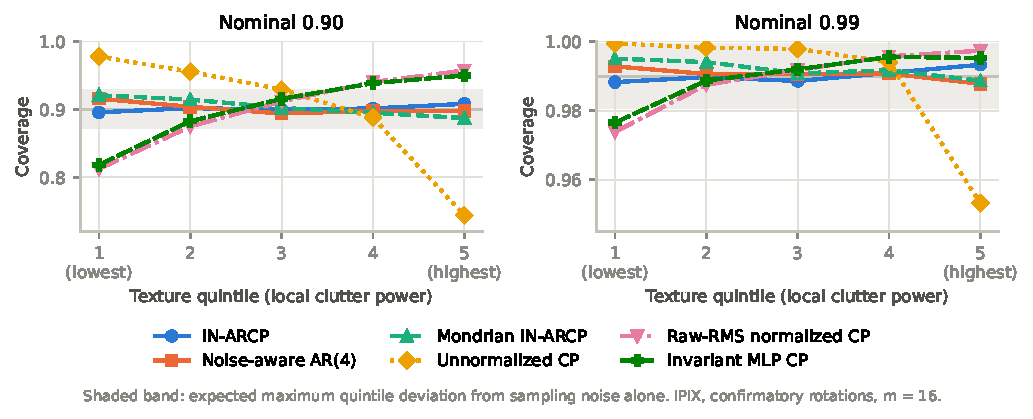
\includegraphics[width=.9\textwidth]{fig_texture_conditional.pdf}
\caption{Coverage by texture quintile on IPIX (confirmatory rotations, $m=16$). Texture is proxied by the local clutter power ($\pm1024$ pulses, excluding the episode).}
\label{fig:texture}
\end{figure*}
The innovation-normalized family stays close to, though above, the sampling-noise reference (Fig.~\ref{fig:texture}): maximum quintile deviations are \MaxdevINOnemSixteenA{} (IN-ARCP), \MaxdevINFourmSixteenA{} (AR(4)) and \MaxdevNAFourmSixteenA{} (NA-AR(4)) against \RefINOnemSixteenA. Unnormalized conformal fails at high texture (\CurveHighUmSixteenA{} in the top quintile; deviation \MaxdevUmSixteenA). Raw-RMS normalization and the invariant neural centre are amplitude-equivariant yet tilt strongly (\MaxdevRMSmSixteenA{} and \MaxdevMLPmSixteenA): equivariance alone would suffice in a pure scale mixture, so real clutter departs from that model, and innovation normalization is what keeps the score approximately pivotal. Mondrian tilts in the predicted direction (\CurveLowMONmSixteenA{} to \CurveHighMONmSixteenA). The pre-specified $\pm512$ and $\pm2048$ proxy windows give the same ranking (Supplementary Material). In detection terms, at a design false-alarm probability of 0.01 the measured false-alarm rate of IN-ARCP ranges from \QPfaINMin{} to \QPfaINMax{} across texture quintiles, a factor of \QPfaINSpread{} (NA-AR(4): \QPfaNAFourSpread), against \QPfaUMin--\QPfaUMax{} (a factor of \QPfaUSpread) for unnormalized conformal prediction, \QPfaRMSSpread{} for raw-RMS normalization and \QPfaMLPSpread{} for the neural centre. The innovation-normalized detectors are therefore approximately, though not exactly, CFAR across clutter power on real clutter.

\subsection{Detection of a target appearing in the predicted pulse}
\begin{figure}[!t]
\centering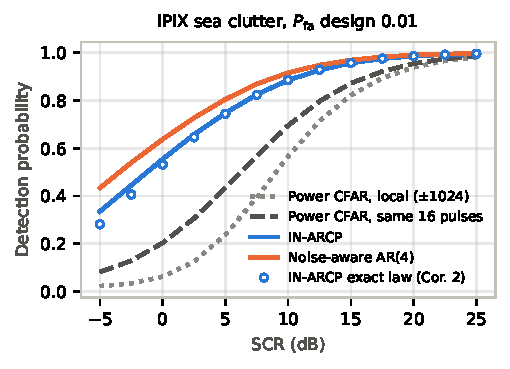
\includegraphics[width=\columnwidth]{fig_detection_col.pdf}
\caption{Detection of Swerling-1 targets injected into the predicted sample of \DetNTest{} real IPIX test episodes (confirmatory units, $m=16$). Thresholds are the clean-data conformal ones. Circles: exact law of Corollary~\ref{cor:detect} evaluated with the clutter+noise model fitted on each unit's training third, without test outcomes.}
\label{fig:detect}
\end{figure}
\begin{table}[!t]
\centering\footnotesize
\caption{SCR (dB) needed for $P_{\rm d}=0.5$ and $0.9$ at $P_{\rm fa}=0.01$ on IPIX, and gain over the power-only detectors (95\% day-cluster intervals).}
\label{tab:detect}
\setlength{\tabcolsep}{3pt}
\begin{tabular}{lccc}
\toprule
 & IN-ARCP & IN AR(4) & NA-AR(4)\\
\midrule
SCR for $P_{\rm d}=0.5$ & \DetINScrHalf & \DetINFourScrHalf & \DetNAFourScrHalf\\
\quad gain vs CA16 & \DetINGainCAHalf{} [\DetINGainCALoHalf, \DetINGainCAHiHalf] & \DetINFourGainCAHalf{} [\DetINFourGainCALoHalf, \DetINFourGainCAHiHalf] & \DetNAFourGainCAHalf{} [\DetNAFourGainCALoHalf, \DetNAFourGainCAHiHalf]\\
\quad gain vs CAloc & \DetINGainLocHalf{} [\DetINGainLocLoHalf, \DetINGainLocHiHalf] & \DetINFourGainLocHalf{} [\DetINFourGainLocLoHalf, \DetINFourGainLocHiHalf] & \DetNAFourGainLocHalf{} [\DetNAFourGainLocLoHalf, \DetNAFourGainLocHiHalf]\\
SCR for $P_{\rm d}=0.9$ & \DetINScrNinety & \DetINFourScrNinety & \DetNAFourScrNinety\\
\quad gain vs CA16 & \DetINGainCANinety{} [\DetINGainCALoNinety, \DetINGainCAHiNinety] & \DetINFourGainCANinety{} [\DetINFourGainCALoNinety, \DetINFourGainCAHiNinety] & \DetNAFourGainCANinety{} [\DetNAFourGainCALoNinety, \DetNAFourGainCAHiNinety]\\
\bottomrule
\end{tabular}
\end{table}
At a design false-alarm probability of 0.01 the measured rates on real clutter are \DetPfaINOne{} (IN-ARCP), \DetPfaNAFour{} (NA-AR(4)), \DetPfaCASixteen{} (CA16) and \DetPfaCAloc{} (CAloc). Fig.~\ref{fig:detect} and Table~\ref{tab:detect} show the detection performance. IN-ARCP needs \DetINGainCAHalf~dB less SCR than power-only detection on the same pulses and \DetINGainLocHalf~dB less than the long-window power detector for $P_{\rm d}=0.5$; NA-AR(4) adds about 1~dB at $P_{\rm d}=0.5$ and 2~dB at $P_{\rm d}=0.9$. The exact law predicts the IN-ARCP detection probability with a mean absolute error of \DetMae{} per unit and SCR (\DetMaePooled{} for the pooled curve), and the SCR needed for $P_{\rm d}=0.5$ within \DetScrErrAbs~dB per unit on average. The clutter-only whitening factor $10\log_{10}(1-|\rho|^2)^{-1}$ would promise \DetNaiveGain~dB; the noise-aware law accounts for the smaller measured gain, as Proposition~\ref{prop:gain} predicts. This is the whitening gain of the prediction-error structure, not a product of conformal calibration: the Gaussian threshold of IN-ARCP (G1) attains the same sensitivity at a similar false-alarm rate. What calibration contributes is the false-alarm budget where the Gaussian threshold fails. The Gaussian plug-in of NA-AR(4) appears more sensitive, but only because it exceeds the budget (\DetPfaNAFourG{} at a design of 0.01 and \DetPfaNAFourGmilli{} at 0.001); with conformal calibration the budget is met and NA-AR(4) still adds 1--2~dB. At $P_{\rm fa}=0.001$ Mondrian calibration has too few calibration episodes per bin and never detects.

\subsection{Persistent targets after onset}\label{sec:onset}
\begin{figure}[!t]
\centering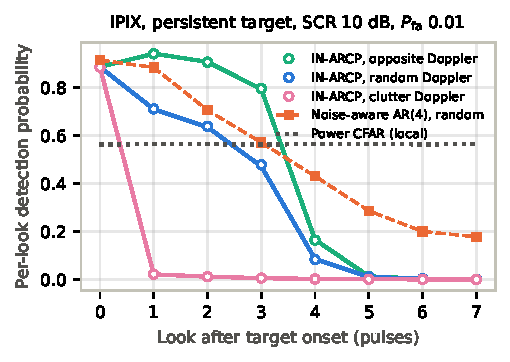
\includegraphics[width=\columnwidth]{fig_onset_col.pdf}
\caption{Per-look detection probability after the onset of a persistent Swerling-1 target on IPIX (SCR 10~dB, per-look $P_{\rm fa}$ design 0.01, \DetNTest{} onset segments). Markers: measured; lines: exact law of Corollary~\ref{cor:detect} with the onset signature, evaluated from the training and calibration thirds only (exploratory).}
\label{fig:onset}
\end{figure}
A real target that appears in a cell usually stays. Under a second frozen protocol we injected persistent Swerling-1 targets with random Doppler at the predicted pulse of each test segment and applied every detector at each of the following eight pulses (Fig.~\ref{fig:onset}). As Proposition~\ref{prop:blind} predicts, IN-ARCP loses the target as it enters the history: at 10~dB SCR its per-look detection probability is \OnLookZero, \OnLookOne, \OnLookTwo, \OnLookThree{} and \OnLookFour{} over the first five looks, while the power detector stays at \OnCAloc. A target at the clutter Doppler is lost after one look (\OnMatchedOne), whereas one at the opposite Doppler survives several (\OnOppOne{} at the second look). NA-AR(4) is less blinded (\OnNALookFour{} at the fifth look). The exact law with the onset signature reproduces these decays, with mean absolute errors of \OnTheoryMaeRand, \OnTheoryMaeMatch{} and \OnTheoryMaeOpp{} per unit and look for random, clutter and opposite Doppler (an exploratory check). The first looks carry the detection: the probability of detecting within eight looks requires \OnGainIN~dB [\OnGainINLo, \OnGainINHi] less SCR with IN-ARCP than with the power detector (\OnGainNAFour~dB for NA-AR(4)), against \OnGainOneIN~dB for one look. We had expected this advantage to fall below 3~dB, and it did not. Because whitened scores give nearly independent false alarms whereas the power detector's false alarms cluster, the probability of at least one false alarm in eight looks is \OnCumPfaIN{} for IN-ARCP and \OnCumPfaCAloc{} for the power detector. In an exploratory comparison at equal dwell false-alarm probability (0.01), with the power detector integrating non-coherently over the eight looks, the advantage remains \DwIN~dB [\DwINLo, \DwINHi] for integrated IN-ARCP scores and \DwNAFour~dB [\DwNAFourLo, \DwNAFourHi] for NA-AR(4) at $P_{\rm d}=0.5$ (\DwNAFourNinety~dB at $P_{\rm d}=0.9$). Integration barely helps the power detector (from \DwCAlocOne{} to \DwCAlocEight~dB for $P_{\rm d}=0.5$), because sea clutter at 1~kHz pulse repetition is so correlated that eight pulses give it few independent looks. Coherent Doppler processing over a full interval, the standard detector for targets that persist, was not part of this comparison.

\subsection{Day transfer, coverage prediction and online calibration}
Across days the width gains largely disappear (NA-AR(4) ratio \TrRatioNAFour; full table in the Supplementary Material), consistent with the documented nonstationarity of sea clutter and IPIX Doppler spectra \cite{greco2010,rosenberg2017}. The innovation-normalized family is the most robust: the worst held-out day covers \TrWorstINOne{} for IN-ARCP, against \TrWorstNAFour{} for NA-AR(4) and \TrWorstMLP{} for the neural centre. The exact law predicts each held-out day's IN-ARCP coverage from its training third, with mean absolute error \CFiveMaeA{} (\CFiveNaiveA{} for the nominal value) at 0.90. With online feedback, ACI ($\gamma=0.02$) raises the worst held-out day from \ACIWorstSplit{} to \ACIWorst{} at a radius ratio of \ACIRadius{} and reduces the texture deviation from \ACIDevSplit{} to \ACIDev; within sessions it matches split calibration (\ACIWithin{} vs \ACIWithinSplit). Innovation normalization and online calibration are therefore complementary.

\subsection{Second radar: 77 GHz ground clutter}\label{sec:jku}
\begin{figure}[!t]
\centering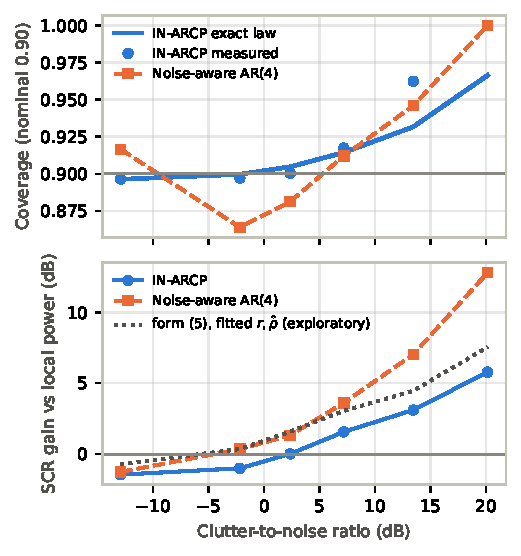
\includegraphics[width=\columnwidth]{fig_jku_col.pdf}
\caption{Second radar (77~GHz FMCW, \JNTest{} million test episodes). Top: coverage by clutter-to-noise class; the line is the exact law. Bottom: SCR gain over the local power detector at $P_{\rm fa}=0.01$, $P_{\rm d}=0.5$, and \eqref{eq:gin} evaluated with the fitted $r$ and $\widehat\rho$ (exploratory).}
\label{fig:jku}
\end{figure}
The parking-lot scene spans CNRs from below $-5$~dB to about 20~dB across range bins, which tests the thermal-noise statements directly (Fig.~\ref{fig:jku}). All conformal methods have marginal coverage within 0.001 of nominal. IN-ARCP coverage rises from \JInLow{} in noise-dominated cells to \JInHigh{} at 10--20~dB CNR, and the exact law of Corollary~\ref{cor:texture} predicts the class coverages with mean absolute error \JMae{} at 0.90 (\JMaeB{} at 0.99; largest error 0.03, at the highest class). Unnormalized conformal coverage collapses from \JULow{} to \JUHigh{} across the same classes. For injected targets, the IN-ARCP gain over the local power detector is \JINGainLow~dB (a loss) in the noise-dominated class, about zero near 0--5~dB and \JINGainHigh~dB at 10--20~dB, following the sign of \eqref{eq:gin}. Evaluated with each unit's fitted $r$ and $\widehat\rho$ (an exploratory check), \eqref{eq:gin} reproduces the trend, from \JGenLow{} to \JGenHigh~dB against \JINGainLow{} to \JMeasTop~dB measured. The remaining optimism of about 1.5~dB is consistent with the finite-history scale estimation that the long-history form ignores. In strong-clutter cells all detectors, IN-ARCP included, run below their design false-alarm rate, because static clutter barely fluctuates. NA-AR(4) avoids most of the low-CNR loss and gains up to \JNAFourGainHigh~dB, better than IN-ARCP in every class. Its CNR-conditional coverage deviation is \JDevNAFour{} against \JDevIN{} for IN-ARCP, but NA-AR(1) is not flatter (\JDevNAOne). Applied to a second run with a corner reflector and an unsynchronized interferer, IN-ARCP keeps \JFourIN{} coverage on clean chirps (NA-AR(4) \JFourNAFour), and interference-hit chirps roughly double its exceedance rate (coverage \JFourHit).

\section{Discussion}
\subsection{What the evidence supports}
\begin{itemize}[leftmargin=*,itemsep=1pt]
\item \textbf{False-alarm control.} On two radars, innovation normalization is what keeps the exceedance rate close to constant across clutter power (a spread of \QPfaINSpread{} against \QPfaUSpread{} on IPIX); amplitude equivariance alone does not, and unnormalized conformal prediction is not CFAR.
\item \textbf{Onset screening.} Within this budget the disc realizes the whitening gain of correlated sea clutter for new returns: about 10~dB over power detection in the first look, retained over an eight-pulse dwell. The gain belongs to the prediction-error structure; calibration keeps it within the budget.
\item \textbf{Richer models.} The noise-aware normalization shortens the regions by about a tenth and adds 1--5~dB of sensitivity, most at high detection probability over a dwell. Only conformal calibration makes it usable, because its Gaussian plug-in breaks the false-alarm budget.
\item \textbf{Exact laws.} They predict coverage across the CNR on two radars, detection probability, its decay after onset, and cross-day coverage.
\end{itemize}

\subsection{Limitations}
\begin{itemize}[leftmargin=*,itemsep=1pt]
\item \textbf{Data.} The sea-clutter evidence comes from one radar and one campaign (14 sessions on six days); the second radar is a static ground scene. Other sea-clutter databases \cite{dewind2010csir} are needed to establish generality across sea states and radars.
\item \textbf{Targets and baselines.} Targets were injected into real clutter. Once a strong target has filled the history it is invisible to the history-normalized score (Proposition~\ref{prop:blind}). Coherent Doppler detection over a full interval, the natural detector for persistent Doppler-separated targets, was not compared; the disc is a complement for new returns, not a replacement. The equal-dwell comparison and the exact-law checks after onset are exploratory.
\item \textbf{Dependence.} Within-session coverage relies on approximate exchangeability \cite{barber2023}; day transfer and ACI are the stricter and the practical safeguards.
\item \textbf{Transfer of the noise-aware model.} Its width and sensitivity gains require same-session training data; across days and measurements IN-ARCP is the safer default. On static ground clutter its CNR-conditional coverage is only partly flatter.
\item \textbf{Texture proxy and proofs.} The texture is proxied, not observed. The noise-aware score is only approximately pivotal; Proposition~\ref{prop:mondrian} is proved for population bins, Proposition~\ref{prop:gain} for a long history, and monotonicity of the CNR-conditional coverage curve remains open.
\end{itemize}

\section{Conclusion}
Innovation normalization makes split-conformal prediction discs texture-conditionally valid in pure compound-Gaussian clutter and keeps them close to that target on real clutter from two radars. Read as detectors of new returns, the discs keep their false-alarm budget across clutter power and realize the whitening gain of correlated sea clutter, about 10~dB over power detection at onset and over an eight-pulse dwell. Exact quadratic-form laws, the CFAR false-alarm law read as coverage, predict their coverage, their detection probability and its decay after onset, and closed forms show how thermal noise caps the gain. Conformal calibration is what lets a richer noise-aware clutter model add sensitivity without breaking the false-alarm budget. Combining the screen with coherent Doppler detection of persistent targets, reference-cell normalization, online operation and further sea-clutter databases remain open.

\appendices
\section{Proof of Proposition~\ref{prop:law}}\label{app:law}
Write $X=\Sigma^{1/2}\xi$ with $\xi\sim\mathcal{CN}(0,I)$. The event is $\{|b^{\mathsf T}X|^2\le q^2s(H)^2\}=\{X^{\mathsf H}M_qX\le0\}$, and after diagonalizing $\Sigma^{1/2}M_q\Sigma^{1/2}$ we have $X^{\mathsf H}M_qX=\sum_k\lambda_kE_k$ with $E_k$ independent standard exponentials. The matrix $M_q$ is the difference of a rank-one positive semidefinite matrix whose range has a nonzero response coordinate and a matrix that is negative definite on the history coordinates, so it has one positive and $m$ negative eigenvalues. By Sylvester's law of inertia $\Sigma^{1/2}M_q\Sigma^{1/2}$ has the same inertia. The characteristic function of $\sum_k\lambda_kE_k$ is $\prod_k(1-\mathrm i t\lambda_k)^{-1}$; partial fractions give the density $\sum_j|\lambda_j|^{-1}e^{-x/\lambda_j}\mathbf 1\{x/\lambda_j>0\}\prod_{k\ne j}\lambda_j/(\lambda_j-\lambda_k)$ for distinct eigenvalues \cite{alnaffouri2016}. Integrating over $x>0$ leaves only the term of $\lambda_+$, which is the probability that the form is positive, and \eqref{eq:exactlaw} follows.

\section{Proofs of Corollary~\ref{cor:detect} and Propositions~\ref{prop:gain} and~\ref{prop:blind}}\label{app:detect}
\emph{Corollary~\ref{cor:detect}.} Conditional on the texture, a Swerling-1 target $\sqrt{SP}\,g\,v$ with $g\sim\mathcal{CN}(0,1)$ independent of the clutter makes the episode $\mathcal{CN}(0,\Sigma+SP\,vv^{\mathsf H})$, so Proposition~\ref{prop:law} applies with this covariance. For pure AR(1) clutter of power $\sigma^2$ at $r=\rho$, $Y-\rho H_m=E+A$ with $E\sim\mathcal{CN}(0,\sigma^2(1-|\rho|^2))$ and $A\sim\mathcal{CN}(0,S\sigma^2)$ independent of $H$, and $m\,s_\rho(H)^2/(\sigma^2(1-|\rho|^2))=\|W_\rho H\|^2/(\sigma^2(1-|\rho|^2))$ is a sum of $m$ independent unit exponentials. Hence $P_{\rm d}=\mathbb E\exp\{-q^2s_\rho^2/(\sigma^2(1-|\rho|^2+S))\}$, which is the Gamma moment-generating function in \eqref{eq:pdclosed}.

\emph{Proposition~\ref{prop:gain}.} If $e\sim\mathcal{CN}(0,v)$ and a Swerling-1 target of power $SP$ is added, a threshold test on $|e|^2/v$ at false-alarm probability $\alpha$ detects with probability $\alpha^{1/(1+SP/v)}$, while the power-only test on $|Y|^2/P$ detects with $\alpha^{1/(1+S)}$; equal $P_{\rm d}$ therefore requires SCRs in the ratio $G=P/v$. For the centre $rH_m$ under \eqref{eq:r7model} with AR(1) speckle, $v=\nu\{c(1+|r|^2-2\Re\,\bar r\rho)+1+|r|^2\}$, which gives \eqref{eq:gin}. For the optimal predictor from the infinite past, $v$ is the one-step prediction-error variance of the AR(1)-plus-white-noise process, $\exp\{\int\log f\}$ by the Kolmogorov--Szeg\H{o} formula \cite{brockwell1991}. With $f(\omega)=\nu\{c(1-|\rho|^2)+|1-\rho e^{-j\omega}|^2\}/|1-\rho e^{-j\omega}|^2$, the denominator contributes zero, and the numerator factorizes as $\nu K|1-\beta' e^{-j\omega}|^2$ with $K(1+|\beta'|^2)=\beta$, $K\beta'=\rho$ and $|\beta'|<1$, which gives $v=\nu K$ and \eqref{eq:gopt}. Because the optimal predictor's error variance is at most that of any linear predictor, including $0$ and $rH_m$, $G_{\rm opt}\ge\max\{1,G_{\rm IN}\}$.

\emph{Proposition~\ref{prop:blind}.} The IN-ARCP score is homogeneous of degree zero, so its value at $X=\sigma Z+Au$, with $u=(e^{j\omega t})_t$, equals its value at $\sigma Z/A+u$, which tends to its value at $u$ as $|A|\to\infty$ by continuity, since $s_r(u)>0$. At $u$ the numerator is $|1-re^{-j\omega}|$ and $m\,s_r(u)^2=(1-|r|^2)+(m-1)|1-re^{-j\omega}|^2$, which gives the limit; it is at most $\sqrt{m/(m-1)}$ because $1-|r|^2\ge0$. If $\widehat q$ exceeds the limit, the score eventually stays below $\widehat q$, and dominated convergence gives $P_{\rm d}\to0$. \hfill$\blacksquare$

\section{Proof of Proposition~\ref{prop:mondrian}}\label{app:mondrian}
Write $t=T(Z_H)$, so that the observed statistic is $T(X_H)=\sigma t$ and $S(X)=S(Z)$. For bin $b$ let $w_b(t)=\PP\{\sigma t\in B_b\}$. Since $\sigma$ is independent of $Z$, for every $x$
\begin{equation}
\PP\{S\le x,\ \sigma t\in B_b\}=\mathbb E\big[\varphi_x(t)\,w_b(t)\big],
\label{eq:app1}
\end{equation}
where $\varphi_x(t)=\PP\{S\le x\mid t\}$.
(i) If $S$ is independent of $t$, then $\varphi_x\equiv F_S(x)$, every bin-conditional law of $S$ equals $F_S$, all $q_b$ equal $F_S^{-1}(1-\alpha)$ and $\mathcal C(\sigma)=1-\alpha$.

(ii) Let $x_0=F_S^{-1}(1-\alpha)$. For the top bin, $w_K(t)=\PP\{\sigma\ge e_{K-1}/t\}$ is nondecreasing in $t$. Because $T$ is continuous, positive and homogeneous and $Z_H$ has full support, $t$ has full support on $(0,\infty)$; as $e_{K-1}/t$ then ranges over $(0,\infty)$ and $G$ is non-degenerate, $w_K(t)$ is not almost surely constant. By assumption $\varphi_{x_0}$ is strictly increasing. Let $t'$ be an independent copy of $t$, $\Delta_\varphi=\varphi_{x_0}(t)-\varphi_{x_0}(t')$ and $\Delta_w=w_K(t)-w_K(t')$. Then
\[
\operatorname{Cov}\{\varphi_{x_0}(t),w_K(t)\}=\tfrac12\,\mathbb E[\Delta_\varphi\Delta_w]>0,
\]
because $\Delta_\varphi\Delta_w\ge0$, with strict inequality on the event $\{w_K(t)\ne w_K(t')\}$, which has positive probability. By \eqref{eq:app1},
$\PP\{S\le x_0\mid\sigma t\in B_K\}=\mathbb E[\varphi_{x_0}w_K]/\mathbb E[w_K]>\mathbb E[\varphi_{x_0}]=1-\alpha$.
The bin-conditional distribution function of $S$ is continuous, so there is $x_1<x_0$ at which it still exceeds $1-\alpha$; hence $q_K\le x_1<x_0$ and, $F_S$ being strictly increasing, $F_S(q_K)<1-\alpha$. For the bottom bin, $w_1(t)=\PP\{\sigma<e_1/t\}$ is nonincreasing, the covariance is negative, and the same steps give $q_1>x_0$ and $F_S(q_1)>1-\alpha$.

The coverage at texture $\sigma$ is $\mathcal C(\sigma)=\sum_b\PP\{S\le q_b,\ \sigma t\in B_b\}$. As $\sigma\to\infty$, $\sigma t\to\infty$ almost surely, so $\mathbf 1\{\sigma t\in B_K\}\to1$ and, by dominated convergence, $\mathcal C(\sigma)\to F_S(q_K)$; as $\sigma\to0$, $\mathcal C(\sigma)\to F_S(q_1)$. An unbinned threshold $q$ gives $\mathcal C(\sigma)=F_S(q)$ for every $\sigma$.

Finally, for IN-ARCP at $r=\rho$ and $T=s_\rho$, $S=|E|/t$ with the innovation $E$ independent of $Z_H$, so $\varphi_x(t)=\PP\{|E|\le xt\}$ is strictly increasing in $t$, which is condition (ii). \hfill$\blacksquare$

\section*{Code and Data Availability}
Code, the four frozen protocols with their hashes, per-episode outcome hashes and figure scripts are in the project repository, https://github.com/razaumair2203-ux/inarcp. The IPIX data are publicly available from McMaster University \cite{ipixweb}, and the 77~GHz data from Zenodo \cite{jku2026}.

\section*{Acknowledgment}
The authors acknowledge the McMaster University IPIX radar group and L.~Rienessl and R.~Feger (Johannes Kepler University Linz) for making their radar data openly available. Generative AI tools were used in this work. OpenAI Codex assisted earlier versions with manuscript editing, literature organization, and implementation and verification code. Anthropic Claude assisted with literature checks, derivations and their numerical verification, implementation, the design and execution of the real-data and synthetic studies, and drafting of all sections. \textbf{[AUTHORS: replace this bracket with a statement of which derivations, analyses and text the authors independently verified.]} The authors take full responsibility for the content.

\bibliographystyle{IEEEtran}
\bibliography{references}

\end{document}
